\graphicspath{ {./ThesisFigures/} }

	\tableofcontents
	
	%\newpage
	
	\pagestyle{fancy}
	%Abbreviations used by fancyhdr:
	%E Even page
	%O Odd page
	%L Left field
	%C Center field
	%R Right field
	%H Header
	%F Footer
	\fancyhead{} % clear all header fields
	\fancyfoot{} % clear all footer fields
	\renewcommand{\headrulewidth}{0.4pt}
	\renewcommand{\footrulewidth}{0.4pt}
	
	\fancyhead[L]{\rightmark}
	\fancyfoot[C]{\thepage}
	\fancyhead[R]{T.P.A. Beishuizen}
	
	
	\clearpage
	
	\newpage
	\section{Introduction}
	\label{sec:Introduction}
	
	% Quick explanation for biomedical data
	Many biomedical datasets are created to use for expansion of biomedical knowledge and improvement of healthcare. Biomedical data is a generalizing term that describes multiple data types\cite{gehlenborg2010visualization}. Examples of biomedical data are micro-array data\cite{brazma2001minimum}, mass spectrometry data\cite{cottrell1999probability, dettmer2007mass} and nuclear magnetic resonance data\cite{capitani2017nuclear}, but also clinically derived data\cite{liu2012data, sittig2008grand}. From a bio-informatics perspective these biomedical data types vary significantly\cite{gehlenborg2010visualization} and therefore extracting information out of biomedical data is not a trivial task. A framework for biomedical data analysis can help guiding biomedical engineers in their process of information extraction from their biomedical datasets. The framework can provide different options in processing the data, taking into account common dataset issues\cite{bertolazzi2008logic, piatetsky2003microarray,lommen2009metalign} and approaches to reach a certain goal\cite{holzinger2014knowledge, wilkins2009proteomics}. Such frameworks are proposed and discussed, however mainly focus on the integration of databases\cite{teodoro2009biomedical, doi:10.1093/nar/gkm1037}, are made specifically for one research area\cite{sturn2002genesis, karnovsky2011metscape, tabas2012genecodis3} or are limited to one specific type of analysis\cite{faul2007g}. A framework that combines database integration, multiple research areas and multiple types of data analysis would be very beneficial for biomedical engineers, guiding them through their biomedical data analysis projects.
	
	% Topic dimensionality reduction
	For such a framework dimensionality reduction is important. Some biomedical datasets contain a high number of features, whereas only a selection of those features are interesting. Therefore especially dimensionality reduction based on feature selection is important. Multiple projects attempted to reduce the number of features\cite{baumgartner2006data, welthagen2005comprehensive} which resulted in multiple algorithm proposals for future research\cite{lim2003planar, peng2010novel, biesiada2007feature, ding2005minimum} and tests on their performance\cite{catal2009investigating, liu2002comparative}. Basic feature selection algorithms should be present in the framework and are therefore tested on the available data sets. Therefore the research goal is \emph{to evaluate the performance of feature selection methods and make a choice on which methods should be added to the framework}. In this document we therefore present several of those algorithms and test their quality.
	
	% Data sets	
	Four data sets were used as a case study for the feature selection algorithms. Two sets are micro-array datasets that are used for research on psoriasis\cite{nair2009genome, suarez2012expanding, bigler2013cross, yao2008type} and cancer\cite{wojnarski2010rsctc}. Two other sets are mass spectrometry data sets, used for research on cancer\cite{NIPS2004_2728} and micro organisms\cite{doi:10.1093/bioinformatics/btu022}. These four datasets all have a high number of features varying from 1000 to 54675 features with a number of samples varying from 200 to 580 samples. All of these datasets are based on classification as tests are done for different test subject groups, therefore the focus on feature selection algorithms will also be based on on classification. Many features are expected to be irrelevant in this classification and therefore could be removed with feature selection.	
	
	\newpage
	\section{Background}
	\label{sec:Background}
	
	% Introduction background & layout background
	Before testing several feature selection methods, first the background of the study is explained. Firstly, the datasets used as a case study and their characteristics are briefly given. Secondly, feature selection methods are discussed. Thirdly the concept automated machine learning is discussed as a possible technique to add to the framework, combined with a tool that implements automated machine learning.
	
	\subsection{Datasets}
	\label{subsec:Datasets}
	
	% Introduction
	Four datasets were used to test feature selection algorithms. The micro-array cancer dataset and both mass spectrometry datasets were found with the help of OpenML\cite{OpenML2013}, whereas the psoriasis dataset was proposed by a project based on psoriasis\cite{felix2017dynamic}. All four of these datasets can be used for classification, as all of them were tested on two or multiple test subject groups. Also, all of them have a high number of features from which most are expected to be irrelevant, so classification would benefit from feature reduction. A schematic overview of the datasets is made (Table \ref{tab:DataSetDescriptions}).
	
	\begin{itemize}
		% Psoriasis
		\item \textit{Psoriasis micro-array dataset} \\ This dataset is comprised of five different data sets\cite{nair2009genome, suarez2012expanding, bigler2013cross, yao2008type}. These five different datasets consist of 54675 features, all corresponding to gene expression. Samples were collected from three different test subject groups: affected skin from test subjects suffering from psoriasis (214 samples), unaffected skin from test subjects suffering from psoriasis (209 samples) and skin from healthy test subjects (167 samples). Combining these three samples types gives 580 samples. Since the data comes from five different experiments, the data is normalized for every experiment.
		% Cancer
		\item \textit{Cancer micro-array dataset} \\ This dataset is used in a challenge focussing on classification problems with a low number of samples, but a high number of features.\cite{wojnarski2010rsctc}. It consists of the same number of features as the Psoriasis data set, 54675 features corresponding to gene expression. It also has 383 samples corresponding to nine different test subject groups. The challenge did not provide labels for the test subject groups. Also these groups differ in size, one group corresponding to 150 samples and the others varying from 16 to 47 samples.
		% Arcene
		\item \textit{Cancer mass spectrometry dataset} \\ This dataset was created as a classification problem to distinguish cancer patterns from normal patterns\cite{NIPS2004_2728}. It is created for the 'Neural Information Processing Systems' conference by merging three mass spectrometry datasets. It consists of 10000 features corresponding to either spectra of the mass spectrometry or probe variables without any predictive power. Samples from two groups are taken, from patients with ovarian or prostate cancer and from control patients. No labels are given to the groups, however it is known that one of the groups has 88 samples and the other 112 samples, combined in a total of 200 samples.
		% MicroOrganisms
		\item \textit{Micro organisms mass spectrometry dataset} \\ This dataset is created to back up a proposed method for routinely performing direct mass spectrometry based bacterial species identification\cite{doi:10.1093/bioinformatics/btu022}. It consists of 1300 features corresponding to different spectra of the mass spectrometry data and 20 test subject groups corresponding to Gram positive and negative bacterial species. Gram classification is a result of a Gram stain test\cite{madigan2017brock}. The groups differ in size varying from 11 to 60 samples, making a total of 571 samples.	
	\end{itemize}

	\begin{table}[]
	\centering
	\caption{A schematic overview of the four datasets.}
	\label{tab:DataSetDescriptions}
	\begin{tabular}{ll|llll}
	\textbf{Dataset focus} & \textbf{Data type}                                          & \textbf{Features} & \textbf{Samples} & \textbf{Classes} & \textbf{Remarks}                                                                                                        \\ \hline
	Psoriasis        & Micro-array                                                 & 54675             & 580              & 3                & \begin{tabular}[c]{@{}l@{}}- Derived from five \\ different datasets\cite{nair2009genome, suarez2012expanding, bigler2013cross, yao2008type} \\ -- \end{tabular}                                       \\
	Cancer           & Micro-array                                                 & 54675             & 383              & 9                & \begin{tabular}[c]{@{}l@{}}- Used in a data \\ mining challenge\cite{wojnarski2010rsctc}\end{tabular}                                            \\ \hline
	Cancer           & \begin{tabular}[c]{@{}l@{}}Mass\\ Spectrometry\end{tabular} & 10000             & 200              & 2                & \begin{tabular}[c]{@{}l@{}}- Created for the \\ NIPS conference\cite{NIPS2004_2728}\\ - Several probe \\ features are present \\ -- \end{tabular} \\
	Micro Organisms  & \begin{tabular}[c]{@{}l@{}}Mass\\ Spectrometry\end{tabular} & 1300              & 571              & 20               & \begin{tabular}[c]{@{}l@{}}- Originates from a \\ micro organisms study\cite{doi:10.1093/bioinformatics/btu022}\end{tabular}                                                                                                                       
	\end{tabular}
	\end{table}
		
	\subsection{Feature Selection}
	\label{subsec:FeatureSelection}
	
	% Introduction feature selection
	Feature selection is a way to perform dimensionality reduction. In feature selection a subset of features is chosen to represent the complete sample space\cite{Guyon2006}. Several techniques are available to choose a representation subset and the effectiveness of these techniques is tested multiple times\cite{CATAL20091040, molina2002feature, chandrashekar2014survey}. These techniques can be grouped in accordingly in three different categories: filter methods, wrapper methods and embedded methods\cite{saeys2007review}. Each of these methods is explained in more detail.
	
	% Preprocessing
	Before actually performing feature selection, usually some kind of preparation or preparation is done. This preparation consists of making the data able for feature selection to be possible as well as preprocessing so all features are processed evenly. Common preprocessing steps include hot encoding categorical values and normalization of numerical values:
	
	\begin{itemize}
		\item \textit{Hot encoding}:\\
		Hot encoding is used when numerical, ordinal and categorical values are combined in the dataset. Whereas numerical and ordinal features have numbers as values, categorical features usually correspond to text with no clear order. Hot encoding is used to give numerical values to the features. This is done by creating a new separate feature for every category and differ the values between presence of this category (e.g. the feature value becomes $1$) and absence of this category (e.g. the feature value becomes $0$). An example would be for a patient either undergoing treatment 'A', 'B' or 'C'. The categorical feature 'treatment' then has the options {'A', 'B', 'C'}. After hot encoding the 'treatment' feature is replaced by features 'treatment A', 'treatment B' and 'treatment C', and the values of these features are either $1$ if that treatment is performed or $0$ if that treatment is not performed. This way no ordering is made possible between categories and they are treated evenly.
		\item \textit{Normalization}:\\
		The difference in value size between numerical features can differ greatly. For example, if both the length of a patient's body and tongue are measured, the value of body length is much bigger than the value for tongue length. On top of that the variance in the features body length and tongue length differ in size, too. To prevent this potential bias in data analysis, all features are normalized on both mean and variance. This normalization is usually done in two steps for a feature with mean $\mu_0$ and standard deviation $\sigma_0$: Step one is changing to a mean value $\mu_1$ with value $\mu_1 = 0$ by subtracting all values by the mean $\mu_0$. Step two is to divide all features by the standard deviation $\sigma_0$, so the new standard deviation $\sigma_1$ becomes $\sigma_1 = 1$.
	\end{itemize}

	% Pseudo-algorithms
	Since these filter methods can usually be best explained by showing example algorithms, several pseudo-algorithms were created for visual clarity. Variables used in these algorithms include:
	\begin{itemize}
		\item \textit{$F$}: A list that contains all the features. It is a list of size $m$ with $m$ being the number of features. A subset $x$ of $F$ is written as $F_x$.
		\item \textit{$X$}: A matrix that contains all sample values for every feature. It is an $n$ by $m$ matrix with $n$ being the number of samples and $m$ being the number of features. If the values of a specific feature $f$ or a subset of features $F_x$ are used this is written as $X_f$ and $X_{F_x}$ respectively, hence the column $f$ or columns $F_x$ are selected.
		\item \textit{$y$}: A vector that contains all class labels for every sample. It is a vector of size $n$ with $n$ being the number of samples.
		\item \textit{$\alpha$}: A threshold value used for ranking and evaluation methods to find out whether a feature should be selected or not in feature selection.
		\item \textit{$W$}: Weights given to a feature after training a machine learning algorithm. The weight of feature $f$ or set of features $F_x$ is called $W_f$ and $W_{F_x}$ respectively.
	\end{itemize}
	
	\subsubsection{Filter Methods}
	\label{subsec:FilterMethods}
	
	% Introduction filter methods
	Filter methods are based on giving relative ranks to the features in a feature space. All features are given a value based on their performance and are ranked by those values\cite{Duch2006, saeys2007review}. Several methods are used to rank the features. These methods are usually based on splitting data matrix $X$ twice. First they are split by feature ($X_{f_1}, X_{f_2} ... X_{f_n}$) for computation. Secondly the columns are split by classes $c_1, c_2 ... c_n$ ($X_{f}^{c_1}, X_{f}^{c_2} ... X_{f}^{c_p}$) to distinguish the predictive power between feature for the classes. A ranking method would quantify the significance according to these values. This results in ranking method $R(X_f, y)$ in which sample label $y$ is used to split the data per class. For illustration a ranking method collection is given:
	
	\begin{itemize}
	% T-test binary
	\item \textit{T-test and ANOVA statistics} \\ 
	Statistics can be used to compare groups with each other. In statistics these groups are seen as separate distributions, which may or may not be seen as independent distributions. If there are two groups a t-test can be done to find the chance for these groups to originate form the same distribution\cite{heiberger2004statistical} (Table \ref{tab:IndepTest}), based on computations on their mean and variance. This t-test gives a probability value (p-value) on interval $[0,1]$, representing the chance the two groups originate from the same distribution. The p-value for the datasets is computed by creating a distribution for every class. Every feature is assigned a different p-value using the distributions for the groups.
	The t-test focuses on the difference between two groups and has different formulas to measure it: A paired t-test if the data can be paired between the two classes, an equal variance t-test and an unequal variance t-test for which it is assumed the variances of the two groups are equal or not equal respectively\cite{heiberger2004statistical} (Table \ref{tab:sdyandtcalc}).
	For sample classifications, the groups would consist of samples with the same label. For example, the t-test can be done between group 1 with classification label "patient" and group 2 with label "normal". If the values of a certain feature from these groups are highly unlikely to follow the same distribution, the p-value will be very low and therefore the rank will be higher.
	
	\begin{table}[h!]
		\centering
		\caption{T-test formulas to compute whether two samples are independent by means. 
			The parameters $s_{\Delta\bar{y}}$ and $t_{calc}$ can be three different 
			values (Table \ref{tab:sdyandtcalc})\cite{heiberger2004statistical}. This is calculated with the values for the mean $\mu$, significance level $\alpha$, average $\bar{y}$.}
		\label{tab:IndepTest}
		\begin{tabular}{llllll}
			\hline
			&  & 
			\multicolumn{2}{l}{\textbf{Tests}} & 
			\textbf{Confidence Interval} & \textbf{}               \\ \cline{3-6} 
			\textbf{H0}              & \textbf{H1}              & \textbf{Rejection 
				region}   & $p$-value                      & 
			\textbf{Lower}               & \textbf{Upper}          \\ \hline
			$\mu_1 \leq \mu_2$                  & $\mu_1 > \mu_2$       & 
			$t_{calc} 
			> t_\alpha$       & $P(t > t_{calc})$      & 
			$((\bar{y}_1 
			- \bar{y}_2) - t_\alpha s_{\Delta \bar{y}}$,       & 
			$\infty)$                     \\
			$\mu_1 \geq \mu_2$                  & $\mu_1 < \mu_2$          & 
			$t_{calc} 
			< -t_\alpha$          & $P(t < t_{calc})$         & 
			$(-\infty$,                        & $(\bar{y}_1 - \bar{y}_2) + 
			t_\alpha 
			s_{\Delta \bar{y}})$ \\
			$\mu_1 = \mu_2$                  & $\mu_1 \neq \mu_2$                  
			& 
			$|t_{calc}| > t_{\frac{\alpha}{2}}$     & $P(t >
			|t_{calc}|)$  & $((\bar{y}_1 - \bar{y}_2) - 
			t_{\frac{\alpha}{2}} 
			s_{\Delta\bar{y}}$ 
			,     & $(\bar{y}_1 - \bar{y}_2) + t_{\frac{\alpha}{2}} 
			s_{\Delta 
				\bar{y}})$  
			\\ 
			\hline
		\end{tabular}
	\end{table}
	
	\begin{table}[h!]
		\centering
		\caption{The values of $s_{\Delta\bar{y}}$ and $t_{calc}$ for data sets 
			with common unknown variance, uncommon unknown variance and paired 
			data. \cite{heiberger2004statistical}. This is calculated with the values for the average $\bar{y}$, variance $s$, population size $n$ and average paired data difference $\hat{d}$.}
		\label{tab:sdyandtcalc}
		\begin{tabular}{lll}
			\hline
			\textbf{Data set}  & \textbf{$s_{\Delta\bar{y}}$}     & 
			\textbf{$t_{calc}$}                                                
			\\ \hline
			Common variance    & $s_{\Delta\bar{y}} = s_p \sqrt{\frac{1}{n_1} + 
				\frac{1}{n_2}}$ & 
			$t_{calc} = \frac{\bar{y}_1-\bar{y}_2}{s_p \sqrt{\frac{1}{n_1} + 
					\frac{1}{n_2}}}         $                                      \\
			Different variance & $s_{\Delta\bar{y}} = s_{\bar{y}_1 - 
				\bar{y}_2}$    & 
			$s_{(\bar{y}_1-\bar{y}_2)} =\sqrt{\frac{s^2_1}{n_1} + 
				\frac{s^2_2}{n_2}}$, and $t_{calc} = \frac{\bar{y}_1 - 
				\bar{y}_2}{s_{(\bar{y}_1-\bar{y}_2)}}$ \\
			Paired data        & $s_{\Delta\bar{y}} = \bar{s}_d$           & 
			$s_{\bar{d}} = s_d / \sqrt{n}$, and $t_{calc} 	
			=\frac{\bar{d}}{s_{\bar{d}}}$                                       
			
			
			\\
			\hline
		\end{tabular}
	\end{table}
	
	If there are more than two groups that must be checked whether they are from the same distribution, a t-test cannot be used. In this case the option is availablefor a multiple group testing, also called analysis of variance (ANOVA). ANOVA computes whether not only two, but multiple groups can originate from the same distribution. ANOVA needs equal group sizes, otherwise the results of the tests are less reliable. The less powerful Kruskall Wallis test can be used if this reliability is needed. Another disadvantage is that t-test and ANOVA assumes the groups follow a certain distribution, which might not be the case\cite{heiberger2004statistical}.
	Most analysis tools have a built-in package for statistics that include T-test and ANOVA. An example for this would be the SciPy\cite{jones2014scipy} package for Python.
	
	% Mutual information
	\item \textit{Mutual information} \\
	Mutual information is another way of matching features with the results. The relevance of using one variable to predict the other variable is used in the equation to compute mutual information (Equation \ref{eq:MutualInformation}). In this equation the probability density function $p$ is used to find the mutual information $MI$ between variables $x$ and $y$\cite{peng2005feature}. Mutual information can be used for both classification and regression. It was initially meant for using in communication channels, however its statistical decision making capabilities makes it a good filter method\cite{battiti1994using}.
	For mutual information packages are commonly available as well. An example would be the mutual information methods for discrete and continuous data in Scikit-Learn\cite{pedregosa2011scikit} for Python.
	

	\begin{equation}\label{eq:MutualInformation}
	MI(x, y) = \int \int p(x, y) \log{\frac{p(x, y)}{p(x)p(y)}} dxdy
	\end{equation}
	
	% Correlation
	\item \textit{Correlation} \\
	Correlation, similarly to mutual information, computes the expressibility of two variables for each other. A variable is relevant if it can predict the outcome of the target variable. One way of computing this relevance for a variable $x_i$ of feature $i$ with mean $\bar{x }_i$ and target variable $y_i$ with mean $\bar{y}_i$ is by using the linear correlation coefficient $r$, also known as Pearson' correlation\cite{yu2003feature} (Equation \ref{eq:Correlation}). The correlation filter methods seem to be a good alternative for continuous data, but not for discrete data. With continuous data, the correlation between feature $x$ and the output $y$ is used to compute the ranks\cite{hall2000correlation}.
	Also for correlation methods packages are commonly availabe. An example is Scikit-Learn\cite{pedregosa2011scikit} again for Python.
		
	\begin{equation}\label{eq:Correlation}
	r(x,y) = \frac{\sum_{i}(x_i - \bar{x}_i)(y_i -\bar{y}_i)}{\sum_{i}(x_i - \bar{x}_i)\sum_{i}(y_i -\bar{y}_i)}
	\end{equation}
	
	\end{itemize}
	
	% Feature selection thresholding criteria
	These ranking methods $R$ to rank the features are only the first step in the filter methods. The next step is choose which features to filter out based on $R$. A quick approach would be to choose a number or fraction $n$ and select the top $n$ ranked features from the complete space (Algorithm \ref{alg:FilterTopNAlgorithm}). Another approach would be to use thresholds derived from literature\cite{donoho2008higher} (Algorithm \ref{alg:FilterAlgorithm}). For the t-test, a p-value of $0.05$ is often chosen as an example\cite{storey2003statistical, higgins2003measuring}.
	
	\begin{algorithm}[H]
		\caption{A basic top $n$ filter algorithm\cite{Duch2006}}\label{alg:FilterTopNAlgorithm}
		\begin{algorithmic}[1]
			\Procedure{FilterSelection($X, y, F, R, n$)}{}
			\State $F_{\textit{selected}} \gets \O$ 	\Comment{Start with empty feature set}
			\State $Z \gets \O$							\Comment{Start with empty set of ranking values}
			\For {$f \textbf{ in } F$} 					\Comment{For all features in $F$}
			\State $Z_f \gets R(X_f, y)$ 				\Comment{Compute the ranking value between feature and output} 			
			\State $Z \gets Z \cup \{Z_f\}$ 				\Comment{Add the ranking value to the set of ranking values}
			\EndFor
			\State $\textbf{Sort } F \textbf{ by } Z$ \Comment{Sort the features by their ranking value}
			\State $F_{}selected \gets F_{[1,n]}$ \Comment{Select the top n features from the sorted feature set}
			\State $\textbf{return } F_{\textit{selected}}$
			\EndProcedure
		\end{algorithmic}
	\end{algorithm}	
	
	\begin{algorithm}[H]
		\caption{A basic filter algorithm\cite{Duch2006}}\label{alg:FilterAlgorithm}
		\begin{algorithmic}[1]
			\Procedure{FilterSelection($X, y, F, R, \alpha$)}{}
			\State $F_{\textit{selected}} \gets \O$ 	\Comment{Start with empty feature set}
			\For {$f \textbf{ in } F$} 					\Comment{For all features in $F$}
			\If {$\text{R}(X_f, y) > \alpha$}			\Comment{Check if ranking value is higher than threshold $\alpha$}
			\State $F_{\textit{selected}} \gets F_{\textit{selected}} \cup \{f\}$ \Comment{Add $f$ to selected features}
			\EndIf
			\EndFor
			\State $\textbf{return } F_{\textit{selected}}$
			\EndProcedure
		\end{algorithmic}
	\end{algorithm}
	
	% Advantages, disdavantages filter methods	
	Using filter methods has its advantages and disadvantages. These filter methods are very computationally efficient. Every feature is given a value for its rank and then a subset is selected based on those ranks. These filter methods however do not take into account dependencies between features. These dependencies could make the final feature subset worse, as maybe some features are related. Other methods are better at handling those dependencies\cite{Duch2006, saeys2007review}.
	
	\subsubsection{Wrapper Methods}
	\label{subsec:WrapperMethods}
	
	% Introduction wrapper methods
	Filter methods take into account the direct relation between features and the output classes, whereas wrapper methods focus more on the subsets of features and their ability to classify the data. Wrapper methods try to find the best combination of features to classify the given data and take into account the change when adding or removing features from a candidate subset\cite{Reunanen2006}. Since an exhaustive search of trying out all possible subsets would span a computation time of $2^n$ with $n$ being the number of features\cite{Alsallakh2016PowerSet}. This combinatorial explosion should be avoided and therefore less computationally intensive approximation concepts have been constructed. Three of those concepts are explained, focusing on basic sequential search, extensions of sequential search and stochastic search.
	
	% Evaluation method
	Before explaining the possible wrapper methods, first the evaluation function $J$ should be discussed. To find out which subset of features can classify the data the best way, a function should be used to evaluate the performance of the subset\cite{Reunanen2006}. Evaluation functions can be based on conditional independence\cite{Reunanen2006,tsamardinos2017massively}, showing the difference in performance for a subset with and without a certain feature. Other evaluation functions are based on machine learning techniques\cite{huang2013automated, saeys2007review}, rating the ability to classify the outcome. A good machine learning algorithm that can be used is Naive Bayes, as it is not very affected by conditional dependency\cite{zhang2004optimality}. Several interesting approaches for evaluation functions are shown in maximum relevance, minimum redundancy algorithms\cite{SENAWI201747, el2009new, radovic2017minimum} (MRMR algorithms). In these MRMR algorithms, several different evaluation functions are used based on the ability of features to classify the outcome (relevance) and the presence of correlation between features (redundancy).
	
	\begin{itemize}
		% Sequential search
		\item \textit{Sequential search} \\
		The first concept to be explained is sequential search. This wrapper method tries to improve a candidate subset by evaluating the change of the sequential addition or removal of a specific feature. Therefore, two types of sequential search are possible, known as forward selection and backward selection. Forward selection starts with the empty subset. Every feature is iteratively evaluated and added to the feature subset if the evaluation function shows an increase in prediction. A maximum feature subset selection size $l$  can be defined if needed, as well. The layout of forward selection is shown as a pseudo algorithm (Algorithm \ref{alg:ForwardSelection}) for understanding\cite{Reunanen2006}.
		
		% Backward selection
		Backward selection does the opposite of forward selection. It starts with the complete feature set in which every feature is iteratively evaluated by the evaluation function for its contribution. If the evaluation function shows that its contribution is very small, it is removed. This way only features with a high impact will remain in the subset. The maximum number features that can be removed $r$ can be defined if needed, as well. give can be A layout of backward selection is shown as a pseudo algorithm (Algorithm \ref{alg:BackwardSelection}) for understanding, as well\cite{Reunanen2006}.
		
		% Order discussion
		In both forward and backward selection the sequence order is important. Different feature subsets will be made for different order of features. The ordering can be changed in a specific way if needed. Examples would be using the ranking concepts used by filter methods. Another possibility would be to randomize the order andrun the algorithm multiple times to find the best subset\cite{Reunanen2006}.
		
		% Insert pseudoalgorithm for forward and backward sequential search
		\begin{algorithm}[H]
			\caption{A forward selection sequential search algorithm\cite{Reunanen2006}}\label{alg:ForwardSelection}
			\begin{algorithmic}[1]
				\Procedure{SequentialForwardSelection($X, y, F, J, \alpha, l$)}{}
				\State $F_{\textit{selected}} \gets \O$				\Comment{Start with empty feature set selection}
				\For {$f \textbf{ in } F$}							\Comment{For all features in $F$}
				\If {$J(X_{F_\textit{selected}}, y, X_f) > \alpha$}	\Comment{Check if evaluation is higher than $\alpha$ with feature $f$}
				\State $F_{\textit{selected}} \gets F_{\textit{selected}} \cup \{f\}$	\Comment{Add $f$ to the feature set selection}
				\EndIf
				\If {$\text{length}(F_{\textit{selected}}) = l$}	\Comment{Stop if size of feature set selection has been reached}	
				\State $\textbf{break}$
				\EndIf
				\EndFor
				\State $\textbf{return } F_{\textit{selected}}$
				\EndProcedure
			\end{algorithmic}
		\end{algorithm}
	
		\begin{algorithm}[H]
		\caption{A backward selection sequential search algorithm\cite{Reunanen2006}}\label{alg:BackwardSelection}
		\begin{algorithmic}[1]
				\Procedure{SequentialBackwardSelection($X, y, F, J, \alpha, r$)}{}
				\State $F_{\textit{selected}} \gets F$				\Comment{Start with complete feature set selection}
				\For {$f \textbf{ in } F_{\textit{selected}}$}		\Comment{For all features in $F_{\textit{selected}}$}
				\If {$J(X_{F_{\textit{selected}} \backslash \{f\}} , y, f) < \alpha$} \Comment{Check if evaluation is higher than $\alpha$ without $f$}
				\State $F_{\textit{selected}} \gets F_{\textit{selected}} \backslash \{f\}$ \Comment{Remove $f$ from the feature set selection}
				\EndIf
				\If {$\text{length}(F \backslash F_{\textit{selected}}) = r$} \Comment{Stop if feature removal limit has been reached}
				\State $\textbf{break}$
				\EndIf
				\EndFor
				\State $\textbf{return } F_{\textit{selected}}$
				\EndProcedure
		\end{algorithmic}
		\end{algorithm}
		
		% Extension sequential search
		\item \textit{Sequential search extension} \\
		The two basic sequential search algorithms forward and backward selection can be altered for better use. An intuitive idea would be to combine the two algorithms, creating an algorithm that first selects features with the evaluation function followed by removing them according to the evaluation function or the other way around. Also there is no restriction on only doing one iteration of both forward and backward selection, giving rise to "plus l-take away r" selection (PTA, algorithm \ref{alg:PTA}). $\text{PTA}(l, r)$ adds $l$ features with forward selection and removes $r$ features with backward selection per iteration, eventually converging to an optimum. 
		These found optima in both sequential search algorithms and possible extensions can converge to local optima, beam search is an example that also collects suboptimal branches for possible better optima, instead of only keeping the best possible outcome at all times\cite{Reunanen2006}.
		
		\begin{algorithm}[H]
			\caption{A plus l-take away r sequential search algorithm\cite{Reunanen2006}}\label{alg:PTA}
			\begin{algorithmic}[1]
				\Procedure{PTA($X, y, F, J, \alpha, l, r$)}{}
				\State $F_{\textit{selected}} \gets \O$			\Comment{Start with empty feature set selection}
				\State $i \gets 0$								\Comment{Initialize feature index}
				\While {$i < \text{length}(F)$}					\Comment{Continue while not all features are evaluated}
				\State $\textit{size} \gets \text{length}(F_{\textit{selected}})$ \Comment{Update size of feature set selection}
				\For {$k \textbf{ in } [i, \text{length}(F)]$}	\Comment{For features in $F$ with index higher than $i$}
				\If {$J(X_{F_{\textit{selected}}}, y, X_{F_k}) > \alpha$}	\Comment{Check if evaluation is higher than $\alpha$ with $f$}
				\State $F_{\textit{selected}} \gets F_{\textit{selected}} \cup F_k$ \Comment{Add $f$ to the feature set selection}
				\EndIf
				\State $i \gets k$						\Comment{Update feature index}
				\If {$ \textit{size} + \text{length}(F_{\textit{selected}}) = l$} \Comment{Stop if feature addition limit has been reached}	
				\State $\textbf{break}$
				\EndIf
				\EndFor
				\State $\textit{size} \gets \text{length}(F_{\textit{selected}})$ \Comment{Update size of feature set selection}
				\For {$f \textbf{ in } F_{\textit{selected}}$}	\Comment{For features in $F_{\textit{selected}}$}
				\If {$J(X_{F_{\textit{selected}} \backslash \{f\}}, y, X_f) < \alpha$}	\Comment{Check if evaluation is higher than $\alpha$ without $f$}
				\State $F_{\textit{selected}} \gets F_{\textit{selected}} \backslash \{f\}$ \Comment{Remove $f$ from the feature set selection}
				\EndIf
				\If {$ \textit{size} - \text{length}(F_{\textit{selected}}) = r$} \Comment{Stop if feature removal limit has been reached}	
				\State $\textbf{break}$
				\EndIf
				\EndFor
				\EndWhile
				\State $\textbf{return } F_{\textit{selected}}$
				\EndProcedure
			\end{algorithmic}
		\end{algorithm}
		
		A last example of a sequential search extension is called floating search. Instead of adding and removing a set number of features as in PTA, floating search continues to add and remove features until the best subset is found (Algorithm \ref{alg:FloatingSearch}). Since feature relevance and redundance changes for every new subset, all features are continuously evaluated to find out if they must be added to or removed from the subset. This way an optimal subset can be found\cite{Reunanen2006}.
		
		\begin{algorithm}[h]
		\caption{A floating search algorithm\cite{Reunanen2006}}\label{alg:FloatingSearch}
		\begin{algorithmic}[1]
				\Procedure{FloatingSearchSelection($X, y, F, J, \alpha$)}{}
				\State $F_{\textit{selected}} \gets \O$			\Comment{Start with empty feature set}
				\While {$F_{\textit{selected}} \textbf{ changes}$}	\Comment{Continue while the feature set selection changes}
				\For {$f \textbf{ in } F$}	\Comment{For features in $F$}
				\If {$f \not \in F_{\textit{selected}} \textbf{ and }J(X_{F_{\textit{selected}}}, y, X_f) > \alpha$} \Comment{Check if evaluation is higher than $\alpha$ with feature $f$}
				\State $F_{\textit{selected}} \gets F_{\textit{selected}} \cup \{f\}$ \Comment{Add $f$ to the feature set selection}
				\EndIf
				\EndFor
				\For {$f \textbf{ in } F_{\textit{selected}}$} \Comment{For features in $F_{\textit{selected}}$}
				\If {$J(X_{F_{\textit{selected}} \backslash \{f\}}, y, X_f) < \alpha$} \Comment{Check if evaluation is higher than $\alpha$ without feature $f$}
				\State $F_{\textit{selected}} \gets F_{\textit{selected}} \backslash f$ \Comment{Remove $f$ from the feature set selection}
				\EndIf
				\EndFor
				\EndWhile
				\State $\textbf{return } F_{\textit{selected}}$
				\EndProcedure
			\end{algorithmic}
		\end{algorithm}
		
		% Stochastic search
		\item \textit{Stochastic search} \\
		
		% Intro + Simulated annealing
		Stochastic search uses random mutations in a candidate subset to achieve an optimal subset. One interesting approach of stochastic search is simulated annealing (SA), a search algorithm based on the cooling down of physical matter\cite{kirkpatrick1983optimization}. This search algorithm tries new feature subsets constantly until the temperature is 'cooled down' or an optimal solution is found (Algorithm \ref{alg:SASearch}). This is done by choosing a new feature every time regardless of whether it is in the subset, or not. If adding or removing the new feature improves the performance of the subset, it will be added or removed. If it worsens the subset, it may be added or removed depending on the quality of deterioration and the temperature. The temperature is lowered after a number iterations of adding or removing features, until it is completely 'cooled down' and the final subset had been made.\cite{Reunanen2006} A second example of a stochastic search algorithm is a genetic algorithm, that collects multiple subsets and mutates them in an evolutionary way\cite{Jirapech-Umpai2005}.
		
		\begin{algorithm}[H]
			\caption{Simulated Annealing search algorithm\cite{Reunanen2006}}\label{alg:SASearch}
			\begin{algorithmic}[1]
				\Procedure{SA($X, y, F, J, T_0, T_1, m, v$)}{}
				\State $F_{\textit{selected}} \gets \text{randomSubset}(F)$	\Comment{Start with random feature subset}
				\State $T \gets T_0$			\Comment{Initialize simulation temperature $T$ with $T_0$}
				\While {$T_0 \geq T_1$}			\Comment{While temperature is not cold enough ($T_1$), yet}
				\State $i \gets 0$				\Comment{Initialize counter for not improvements}
				\While {$i < m$}				\Comment{While not improvements is lower than maximum $m$}
				\State $f \gets \text{randomFeature}(F)$	\Comment{Select random feature $f$}
				\If {$f \in F_{\textit{selected}}$}	\Comment{Check if $f$ is in feature set selection}
				\State $F_{\textit{candidate}} \gets  F_{\textit{selected}} \backslash \{f\}$ \Comment{create candidate feature subset selection}
				\State $\Delta = J(X_{F_{\textit{selected}} \backslash \{f\}}, y, X_f)$ \Comment{Calculate evaluation difference without feature $f$}
				\Else	\Comment{Check if $f$ is not in feature set selection}
				\State $F_{\textit{candidate}} \gets  F_{\textit{selected}} \cup \{f\}$	\Comment{create candidate feature subset selection}			
				\State $\Delta = J(X_{F_{\textit{selected}}} , y, X_f)$ \Comment{Calculate evaluation difference with feature $f$}
				\EndIf
				\If {$\Delta > 0$} \Comment{Check if change is positive}
				\State $F_{\textit{selected}} \gets F_{\textit{candidate}}$ \Comment{Use candidate as feature subset selection}
				\Else
				\State $r \gets randomReal(0, 1)$ \Comment{Get a random value $r \in [0, 1]$}
				\If {$r < \text{exp}(-\Delta / T)$}  \Comment{Check if a random change should occur}
				\State $F_{\textit{selected}} \gets F_{\textit{candidate}}$ \Comment{Use candidate as feature subset selection}
				\EndIf
				\State $i \gets i + 1$ \Comment{Increment counter for no improvement}
				\EndIf				
				\EndWhile
				\State $T \gets T \times v$ \Comment{Lower the temperature with $v \in [0,1]$} 
				\EndWhile
				\State $\textbf{return } F_{\textit{selected}}$
				\EndProcedure
			\end{algorithmic}
		\end{algorithm}
		 
	\end{itemize}

	% Advantages/Disadvantages
	The major advantage of using wrapper methods is that it also takes into account possible dependencies between features. The computation time of wrapper methods usually is higher than of filter methods, but still relatively short as it should always converge to an optimum. These optima can be local however, so the result may not be the optimal, due to its greedy character. The stochastic search algorithms provide a way find a global optimum at the cost of being more computationally intensive. Also, these methods are dependent on the evaluation function and are known to be prone for overfitting\cite{Reunanen2006, saeys2007review}.
	
	\subsubsection{Embedded Methods}
	\label{subsec:EmbeddedMethods}
	
	% Introduction Embedded methods
	In both filter and wrapper methods, machine learning plays little to no role in selecting features. Filter methods do not use learning at all and a wrapper method can only use machine learning for the performance of feature subsets. Machine learning however has multiple attributes that can be used directly to select or eliminate features from the ideal feature set selection. Embedded methods combine feature selection with a machine learning algorithm $M$, in contrast of wrapper methods in which these are separated\cite{Lal2006}. Usually this combination involves using the weights given to features by machine learning algorithms\cite{blum1997selection}.
	
	Embedded methods usually solve feature selection by using one of two possible solution. The first solution is based on contribution relaxation minimization and the second solution is based on convex function minimization. Since the theoretical approach of embedded methods can be very computationally intensive, approximations of the minimization problems are given, showing exemplary embedded methods\cite{Lal2006}.
	
	
	\begin{itemize}
		\item \textit{Contribution relaxation minimization} \\
		
		% Explanation contribution relaxation
		Contribution relaxation is based on giving every feature $f$ a contribution factor $\sigma_f \in [0, 1]$. This contribution factor shows the contribution of a feature to the preferred outcome. The final goal is to select a subset of features, though, and not use all features with a contribution factor. To achieve that a minimization function is used in which all contribution factors become $\sigma_f \in \{0, 1\}$. With contribution factors in $\{0, 1\}$, a subset with all features having $\sigma_f = 1$ can be selected as the ideal subset\cite{Lal2006}. 
		
		% Approximation of methods
		The minimization can be implemented with a feature selection method. This method would however be computationally intensive and therefore approximations are used. The most used approximation is similar to the filter methods, ranking each feature and choosing features based on rank. This embedded method is also called a forward selection method. A machine learning algorithm $M$ assigns a weight to each feature, which can be used as a rank (Algorithm \ref{alg:FilterAlgorithm}). The difference between a ranking method $R$ of the filter methods and the weights of a machine learning algorithm $M$ is that $M$ also take into account the dependency between features\cite{Lal2006}.
		
		\begin{algorithm}[H]
			\caption{An embedded forward selection algorithm\cite{Lal2006}}\label{alg:EmbeddedForwardSelectionAlgorithm}
			\begin{algorithmic}[1]
				\Procedure{EmbeddedForwardSelection($X, y, F, M, \alpha$)}{}
				\State $F_{\textit{selected}} \gets \O$ 	\Comment{Start with empty feature set}
				\State $W \gets M(X, y)$					\Comment{Extract the weights for every feature}
				\For {$f \textbf{ in } F$} 					\Comment{For all features in $F$}
				\If {$W_f > \alpha$}			\Comment{Check if weight is higher than threshold $\alpha$}
				\State $F_{\textit{selected}} \gets F_{\textit{selected}} \cup \{f\}$ \Comment{Add $f$ to selected features}
				\EndIf
				\EndFor
				\State $\textbf{return } F_{\textit{selected}}$
				\EndProcedure
			\end{algorithmic}
		\end{algorithm}
		
		\item \textit{Convex function minimization} \\
		
		% Explanation convex function minimization
		The convex function minimization focuses on the trade-off between prediction quality and feature subset size. Convex function minimization combines a loss function, used for quality measurements, with a penalty term for the number of features used. This results checking for which features the quality increase is lower than the penalty term, so it should be removed. There are many different loss functions that can be used for this case, all with their own advantages and disadvantages\cite{Lal2006}.
		
		% Approximation with methods
		For approximation of this minimization, an embedded method closely related to the backward selection wrapper method can be used called Recursive Backward Elimination (RBE, Algorithm \ref{alg:EmbeddedBackwardEliminationAlgorithm}). In RBE a machine learning method gives weights for every feature. The feature with the lowest weight is then compared with a threshold and removed if too low for the threshold. Since weights of a machine learning algorithm change when features are removed, this should be done recursively until no feature can be found any more with a weight lower than the threshold\cite{Lal2006}.
		
		\begin{algorithm}[H]
			\caption{An embedded backward elimination algorithm\cite{Lal2006} }\label{alg:EmbeddedBackwardEliminationAlgorithm}
			\begin{algorithmic}[1]
				\Procedure{RecursiveBackwardElimination($X, y, F, M, \alpha$)}{}
				\State $F_{\textit{selected}} \gets F$ 	\Comment{Start with complete feature set selection}
				\While {$F_{\textit{selected}} \textbf{ changes }$} \Comment{While the feature set selection changes}
				\State $W_{F_{\textit{selected}}} \gets M(X_{F_{\textit{selected}}}, y)$\Comment{Extract the weights for every feature}
				\State $f_{\textit{min}} \gets f \in F_{\textit{selected}} \textbf{ with } W_f = \text{min}(W_{F_{\textit{selected}}})$ \Comment{Find the feature with the lowest weight}
				\If {$W_{f_{\textit{min}}} < \alpha$}	\Comment{Check if weight is lower than threshold $\alpha$}
				\State $F_{\textit{selected}} \gets F_{\textit{selected}} \backslash \{f\}$ \Comment{Remove $f$ from selected features}					
				\EndIf
				\EndWhile
				\State $\textbf{return } F_{\textit{selected}}$
				\EndProcedure
			\end{algorithmic}
		\end{algorithm}
			
	\end{itemize}

	% Examples of weights
	The weights given by machine learning are different for every algorithm. A first and most obvious example of an algorithm giving weights are algorithms based on support vector machines (SVM). The weights given by SVM give the features a contribution factor in the outcome\cite{jong2004feature, prados2004mining, zhang2006recursive, guyon2002gene}. A second example would be using decision trees and random forests. Decision trees use features to reduce the entropy between a set by splitting it in two subsets with a threshold and a feature. These splitting features can be used as a subset to create an effective feature selection outcome\cite{geurts2005proteomic, wu2003comparison, Duch2006}. To overcome an overfitting problem, commonly occuring in decision trees, random forests can be used instead and the best splitting features can be used\cite{liaw2002classification}.

	% \subsection{Feature Extraction}
	% \label{subsec:FeatureExtraction}
	
	% PCA
	% LDA
	
	% extraction algorithms: https://link.springer.com/book/10.1007/978-3-540-35488-8?page=1#toc	
	
	%\subsection{Feature Selection Frameworks}
	%\label{subsec:FeatureSelectionFrameworks}
	
	% https://arxiv.org/pdf/1610.09543.pdf
	
	\subsection{Automated Machine Learning}
	\label{subsec:AutomatedMachineLearning}
	
	% History autoML
	Before automated machine learning (autoML) existed, a dataset was mined by hand. First a preprocessing algorithm was chosen and used to prepare the data. Next a (machine learning) algorithm was chosen to mine the desired results out of the data. At last the hyper-parameters of the chosen algorithm were tuned to optimize the desired results. These three steps are vastly different and significant issues arise when combining these. Several ideas arose to combine the steps, called Combined Algorithm Selection and Hyperparameter optimization (CASH)\cite{thornton2013auto}. After some time, when preprocessing was added in the mix as well, the name autoML was being used\cite{Gijsbers2017Thesis}. The first autoML approach tool was published as \texttt{Auto-WEKA} that focused on classification methods, spanning 2 ensemble methods, 10 meta-methods, 27 base classifiers and their hyperparameter settings\cite{thornton2013auto}. An upgrade was published that added regression and parallellism\cite{kotthoff2016auto}.   
	
	% Introduction to pipelines
	As explained shortly before, to go from data and results several steps must be taken: Preprocessing, algorithm selection and hyperparameter optimization. This sequencing is called a machine learning pipeline. Such a pipeline can consists of zero, one or multiple preprocessing steps for data preparation, can be one of many different machine learning algorithms which on their part have wide ranges for multiple hyper-parameters. The explosion of possible pipelines makes it hard to choose the right one. Knowing successful combinations is useful, however every data set has different features that ask for different pipelines\cite{Gijsbers2017Thesis}.
	
	% Introduction autoML
	AutoML tries to find the best machine learning pipelines to compute which algorithms must be selected, combined with tuning the hyper-parameters and preprocessing. This algorithm selection usually is done in a meta-learning approach, which focuses on finding how the machine learning algorithms perform for a task interval. Hyperparameter optimization has challenges on his own to find the right ones and there are many different approaches to tackle preprocessing. The concept of meta-learning is briefly explained in more detail (Subsection \ref{subsec:Meta-Learning}). Aside from that, a tool that makes use of AutoML, TPOT, is also discussed (Subsection \ref{subsec:TPOT}). 	
	
	
	\subsubsection{Meta-Learning}
	\label{subsec:Meta-Learning}
	
	% Introduction meta-learning
Machine learning algorithms show different behaviour for different tasks. Meta-learning tries to find out how their performance changes between those tasks (Figure \ref{fig:Meta-LearningLayout}). It tries to link the datasets with a suitable algorithm for high performance and tries to improve this performance by finetuning its hyper-parameters. In combination with the machine learning pipelines, meta-learning tries to find the best ones available. Since not only algorithms must be selected, but also hyper-parameters must be optimized and preprocessing must be done, the time and space needed for meta-learning causes a combinatorial explosion. This can be lessened by stopping the investigation of bad pipelines and limiting the range of hyper-parameters, machine learning- and preprocessing algorithms as much as possible. 

\begin{figure}
	\label{fig:Meta-LearningLayout}
	\includegraphics[scale=1]{Meta-LearningLayout.png}
	\caption{A layout of how meta-learning works. 1. Data sets are collected. 2. Meta-data is computed for each dataset. 3. A meta-dataset is created and a meta-model is learned\cite{Gijsbers2017Thesis}.}
\end{figure}

% Meta-features
Features of the meta-learning phenomenon are used to predict the performance. There are three types of these meta-features. The first type is simple, statistical and information-theoretic. They can be a basic feature of the data set, as well as a value after a statistical computation or a specific theoretical value. The second meta-feature type can be called landmarks. Landmarks give the performance of algorithms, how well they are doing with the given data set. The last meta-feature category is model-based. Specific characteristics of the used model can be used as meta-features as well\cite{brazdil1994characterizing, vilalta2004using}.

% Meta-learners
For using those meta-features in picking the best machine learning algorithm meta-learners can be used. Meta-learners are algorithms that choose between the possible choices. There are four ways of doing that. The first is plainly choosing the best algorithm in the set, this choice speeds up the process but is prone to being a bad choice. Second a subset of good algorithms can be chosen, which is slower, but has a higher chance to give a good outcome. Thirdly the algorithms can be ranked, which makes the chance of picking a good algorithm quicker starting at the top. Fourth is to use estimations of performance which gives information expectations over all algorithms\cite{brazdil2009development}.
	
	
	\subsubsection{Tree-based Pipeline Optimization Tool}
	\label{subsec:TPOT}
	
	% Introduction TPOT
	A tool that implements autoML is tree-based pipeline optimization tool (TPOT). It uses the machine learning pipelines and evolutionary optimization to find the best solution for every data set. This evolutionary optimization is done by genetic programming. Genetic programming evolves possible solutions to find a better solution. This evolution is done by first evaluating them and selecting the best ones to continue to the next generation. Then both crossovers between and mutations on possible solutions are performed. After that again evaluation and selection, followed by crossovers and mutations, take place a number of times until a certain quality is found, time has run out or another ending condition has been met.
	
	% TPOT layout
	TPOT makes use of this genetic programming with using the machine learning pipelines in a tree (Figure \ref{fig:MachineLearningPipeline}). TPOT consists of preprocessing and machine learning algorithms, that form the backbone of the pipelines (Table \ref{tab:TPOTAlgorithms}). Their hyper-parameters are the variables. TPOT makes mostly use of the machine learning and preprocessing algorithms of skikit-learn from Python in which it is also written, but also several additional algorithms are present (e.g. a hot encoding algorithm).
	
	\begin{table}[]
		\centering
		\caption{All TPOT Algorithms used for the TPOT classifier function. Not only the algorithms differ, but also the hyper-parameters within these algorithms.}
		\label{tab:TPOTAlgorithms}
		\begin{tabular}{ll|l}
			\textbf{Algorithm type} & \textbf{Specification}  & \textbf{Algorithms}                                                                                                        \\ \hline
			\textbf{Classifier}     & Naïve Bayes             & GaussianNB, BernoulliNB, MultinomialNB                                                                                     \\
			\textbf{}               & Decision Tree           & \begin{tabular}[c]{@{}l@{}}DecisionTree, ExtraTrees, RandomForest, \\ GradientBoosting\end{tabular}                        \\
			\textbf{}               & Nearest Neighbor        & KNeighbors                                                                                                                 \\
			\textbf{}               & Support Vector Machines & LinearSVC                                                                                                                  \\
			\textbf{}               & Logistic Regression     & Logistic Regression                                                                                                        \\ \hline
			\textbf{Preprocessors}  & Scaler                  & \begin{tabular}[c]{@{}l@{}}Binarizer, MaxAbsScaler, MinMaxScaler, \\ Normalizer, RobustScaler, StandardScaler\end{tabular} \\
			\textbf{}               & Feature reduction       & \begin{tabular}[c]{@{}l@{}}PCA, FastICA, RBFSampler, Nystroem,\\ FeatureAgglomeration\end{tabular}                         \\
			\textbf{}               & Feature Modifier        & Polynomial, OneHotEncoder,ZeroCount                                                                                        \\
			\textbf{}               & Feature Selectors       & \begin{tabular}[c]{@{}l@{}}SelectFwe, SelectPercentile, VarianceThreshold, \\ RFE, SelectFromModel\end{tabular}           
		\end{tabular}
	\end{table}
	
	\begin{figure}[h!]
		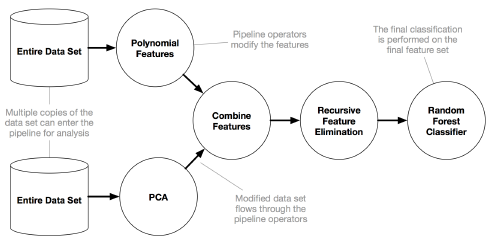
\includegraphics[scale=1]{MachineLearningPipeline.png}
		\caption{An example of a machine learning pipeline in TPOT. It only shows the primitive algorithms and not hyperparameter terminals. At the root is the machine learning algorithm\cite{Gijsbers2017Thesis}.}
		\label{fig:MachineLearningPipeline}
	\end{figure}
	
	% TPOT mutation operators
	TPOT has three different types of mutations within one pipeline.The first one is insertion, inserting a primitive somewhere in the tree. An example would be the insertion of an additional preprocessing algorithm. The second one is replacement, which replaces a random terminal. It can for example change a binary hyper parameter from true to false. The third one is shrinking. A primitive is replaced by a terminal. For example a preprocessing step can be replaced by just raw data. This different mutations can all be seen visually (Figure \ref{fig:TPOTMutations})
	
	\begin{figure}[h!]
		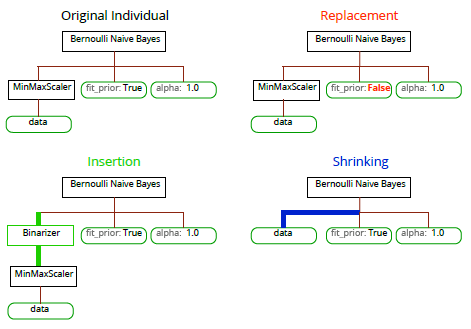
\includegraphics[scale=1]{TPOTMutations.png}
		\caption{Examples of the three mutations in the TPOT algorithm: insertion, replacement and shrinking\cite{Gijsbers2017Thesis}.}
		\label{fig:TPOTMutations}
	\end{figure}
	
	% Crossover
	TPOT also focuses on mutations between two pipelines through the means of crossovers. Between two pipelines, sub-trees and primitives can be changed, given that the both pipelines remain valid (Figure \ref{fig:TPOTCrossover}). Every time a crossover is performed, two separate pipelines are used and changed, creating two new ones.
	
	\begin{figure}[h!]
		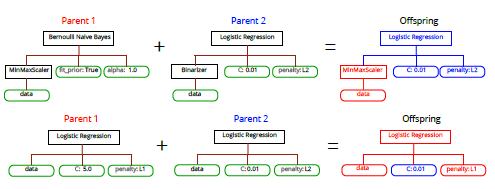
\includegraphics[scale=1]{TPOTCrossover.png}
		\caption{An example of a TPOT crossover\cite{Gijsbers2017Thesis}.}
		\label{fig:TPOTCrossover}
	\end{figure}
	
	% Biomedical preprocessing
	Comparing the possibilities from TPOT and the challenges in biomedical data, it seems that TPOT has some implementations to tackle them. It has several different scalers (StandardScaler, RobustScaler, MinMaxScaler) to tackle feature heterogeneity between different data sets and errors. It also has some feature selection operators to tackle errors (VarianceThreshold, SelectKBest, SelectPercentile). For missing values, the algorithm imputes the median as estimation for the missing value.
	
	\newpage
	\section{Hypotheses}
	\label{sec:hypotheses}
	
	The main goal for this project is to find more insight in feature selection and add that insight to the final framework. Several hypotheses are made before designing experiments to test them and are discussed here:
	
	\begin{enumerate}
		\item \textbf{Optimum in number of selected features} \\
		An optimum should be found in the number of selected features. Whereas using too many features may cause issues for a machine learning algorithms to extract the correct information from them, preserving too few features may result in lost information. Previous research scaled down the number of features from 400 to 96\cite{pazzani1997learning}, 500 to 13 and for even bigger datasets from 5000-100000 features to between 200 and 900 relevant features\cite{chen2006combining}. Interestingly, the number of relevant features was not related to the original feature set size, indicating the optimum to be an absolute number. The value of this absolute optimum is estimated to be lower than 1000, as no study before ever used a lower number of relevant features.
		\item \textbf{Best feature selection methods} \\
		Three types of feature selection methods are discussed, all of them having a their own advantages. Out of these three, the embedded methods are expected to outperform the others. Whereas filter methods are quick and easy, their efficiency should be lower the lower than the other methods. Wrapper methods are more close to trying to find the optimal solution the exhaustive way and therefore are expected to perform the best feature selection at a cost of computation efficiency. At last the embedded methods are expected to be in between of the two. The embedded methods use machine learning methods that are fairly quick and easy to understand to find the results and those machine learning methods somewhat use relative contributions between features. This would mean that embedded methods are quicker and easier than wrapper methods and more efficient than filter methods and therefore combining the best of both.
		\item \textbf{TPOT feature selection integration} \\
		Integration of feature selection in TPOT for the framework can be done in different ways. Two ways are thought to be an addition to the tool. First expanding the number of feature selection methods should improve TPOT in finding better pipelines. Secondly having TPOT start with an initial pool of pipelines including feature selection methods should give it a head-start and therefore be quicker and better and finding good pipelines.		
	\end{enumerate}
	
	\newpage
	\section{Methods}
	\label{sec:Methods}

	% Introduction methods
	For empirical evaluation the collection of feature selection methods experiments are done. The quality of the feature selection is tested by creating a definition of quality first. After that an exploration of feature selection is done with filter methods, followed by comparisons of multiple feature selection methods. The tests are done in Python, using the Anaconda distribution, as with Anaconda external packages can be used quickly. Methods that can be used for feature selection are from the packages scikit-learn\cite{pedregosa2011scikit}, SciPy\cite{jones2014scipy} and NumPy\cite{walt2011numpy}. The four example datasets (subsection \ref{subsec:Datasets}) were used as exemplary datasets for the experiments.
	
	\subsection{Feature Selection Quality}
	\label{subsec:DimensionalityReductionQuality}
	
	% Machine learning for testing
	To find out the quality of the feature selection, multiple machine learning algorithms are used\cite{hall1998practical}.  Classification of the datasets can be done with several machine learning algorithms and validation and tests scores show how well the data can be classified after feature selection. The quality will be described with the accuracy of machine learning algorithms: the number of right classifications divided by the total number of classifications. Five different machine learning classifiers are used from scikit-learn: logistic regression, decision trees, nearest neighbour, support vector machines and Naive Bayes. Better feature selection algorithms have relatively higher accuracy, as they are better at preserving the right features. Since overfitting sometimes happens when fitting data in a machine learning algorithm, both a validation and a test score is computed for the accuracy. For every experiment a training set and a test set is created, making the test set 20\% of the complete dataset. A validation score is computed by using leave one out (scikit-learn) on the training set and a test score is computed by testing the classification score of the test set. Since the samples are not evenly distributed over the classes the precision, recall and F1 scores are also computed to find potential bias in the result.

	% Addition to number of features
	In some cases the quality of the machine learning algorithm lacks a factor of feature subset size. The accuracy in those cases is not sufficient enough to evaluate the result. To incorporate the quality of feature selection a new modified quality term FS\_accuracy is created (Equation \ref{eq:FSAccuracy}). In FS\_accuracy a modified version of the original accuracy is given by first multiplying it by a a factor dependent on the number of features. This factor consists of a constant $\alpha$, a value in range $[0, 1]$ which can be chosen for the influence of the  value that represent the number of features. In practice $\alpha > 0.95$ so the reduction does not have too much influence on the accuracy. An example plot of how the correction factor changes is given (Figure \ref{fig:FSAccuracyPlot}).
	
	\begin{equation*}
	\label{eq:FSAccuracy}
	\text{FS\_accuracy} = \text{accuracy} \times \alpha^{\text{\#features}}
	\end{equation*}
		
		% Insert figures
	\begin{figure}[H]
		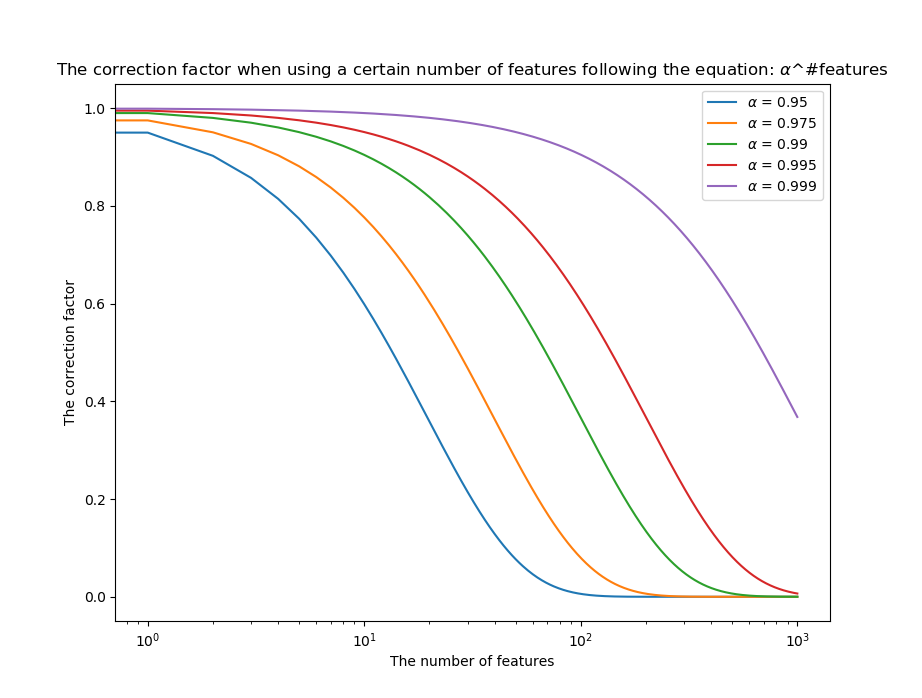
\includegraphics[width=1\textwidth]{FS_accuracy_alpha.png}
		\caption{The correction factor for the FS\_accuracy from Equation \ref{eq:FSAccuracy}. Every graph corresponds to a different value of $\alpha$.}
		\label{fig:FSAccuracyPlot}
	\end{figure}
	
	% Absolute number of features
	The factor $\#features$ is an absolute count, instead of a relative count (for example a percentage of features). The goal of data analysis is the main reason for using an absolute count. In data analysis the number of features that can be relevant are very limited. Useful results need relations between the input and the output, and these relations need to be as simple as possible. If the number of features is relative to the total number of features, the input size can change significantly. Take for example the Micro Organisms and the RSCTC datasets provided for this study (Subsection \ref{subsec:Datasets}). 2\% of the total features would be 26 and 1100 features for these datasets respectively. Whereas relations between 26 features and the output is possible to understand, relations between 1100 features and the output is much harder. Taking an absolute number of features lets you more actively choose for the input size.
	
	% Selection proper alpha
	To put the impact of the FS\_accuracy in perspective, an exemplary figure is made how the outcome is computed (Figure \ref{fig:FSAccuracyExample}). This figure shows the impact on the performance of a method when using a certain number of features. After using a correction factor, a new optimum is created for which the number of features is important. The example (with $\alpha = 0.99$) seems to give a good indication of the desired outcome. For every $10$ features, the FS\_accuracy is reduced by about 10\% (Figure \ref{fig:FSAccuracyPlot}), which meant for the exemplary filter method that for 50 features an optimum was reached (Figure \ref{fig:FSAccuracyExample}). Because of this empirically found desired trade-off, $\alpha = 0.99$ will be chosen in this project when using FS\_accuracy. 
	
	% Insert figures
	\begin{figure}[H]
		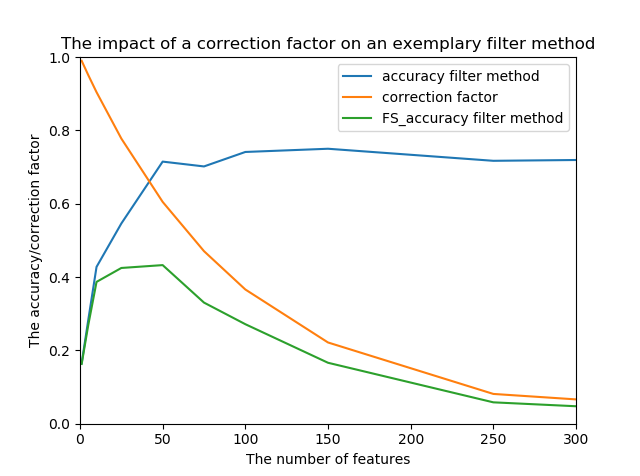
\includegraphics[]{FS_accuracy_example.png}
		\caption{An example of the impact of the correction factor on the accuracy. The shown correction factor uses $\alpha = 0.99$. On the x-axis the number of features is shown and on the y-axis the value for the original accuracy, the correction factor and the FS\_accuracy.}
		\label{fig:FSAccuracyExample}
	\end{figure}
	
	\subsection{Feature Selection Exploration}
	\label{subsec:FeatureSelectionExploration}
	
	% First experiment
	The first set of experiments is used to explore a combination of the basic filter method combined with the quality measurements. The basic filter method algorithm selecting the top $n$ features (Algorithm \ref{alg:FilterTopNAlgorithm}) is used. The changing variables are the dataset, the ranking method, the feature preservation values and the accuracy computation methods (Table \ref{tab:FirstExperimentRequirements}). The range of chosen feature preservation values comes from both its ability to show impact of separate features (more impact from fewer features) and the relevance of keeping that number of features (irrelevant feature selection when having more than 1000 features). All of this together means a total of $4 (\text{datasets}) \times 2 (\text{ranking methods}) \times 11 (\text{top } n \text{ features}) \times 5 (\text{accuracy computation methods}) = 440$ experiments are conducted. These experiments are visualized in eight plots, one plot for every combination of data set and ranking method. These plots then show the change in quality for different number of preserved features.
	
	\begin{table}[]
	\centering
	\caption{The four meta-parameters with their possible values in the first experiment.}
	\label{tab:FirstExperimentRequirements}
	\begin{tabular}{l|ll}
		\textbf{Variable} & \textbf{Description}                                                                              & \textbf{Values}                                                                                                                         \\ \hline
		Dataset           & The datasets used (subsection \ref{subsec:Datasets})                                                                                 & \begin{tabular}[c]{@{}l@{}}Psoriasis\\ RSCTC\\ Arcene\\ Micro-Organisms\\ --\end{tabular}                                               \\
		Ranking method    & \begin{tabular}[c]{@{}l@{}}The method used for ranking \\ the features (subsection \ref{subsec:FilterMethods})\end{tabular}               & \begin{tabular}[c]{@{}l@{}}T-test (SciPy)\\ Mutual Information (scikit-learn)\\ --\end{tabular}                                                                \\
		Feature preservation values & \begin{tabular}[c]{@{}l@{}}The fixed size of the feature subset \\ after feature selection\end{tabular} & \begin{tabular}[c]{@{}l@{}}1, 5, 10, 25, 50, 75, \\ 100, 150, 250, 500, 1000\\ --\end{tabular}                                          \\
		Accuracy computation & \begin{tabular}[c]{@{}l@{}}The machine learning algorithms \\ used to compute accuracy (subsection \ref{subsec:DimensionalityReductionQuality})\end{tabular}   & \begin{tabular}[c]{@{}l@{}}Naive Bayes\\ Logistic Regression\\ Support Vector Machine\\ Decision Tree\\ Nearest Neighbours\end{tabular}
	\end{tabular}
	\end{table}
	
	\subsection{Feature Selection Algorithms Evaluation}
	\label{subsec:FeatureSelectionAlgorithmsEvaluation}

	% Second experiment
	The second set of experiments compares the feature selection methods in both feature selection and quality. For this experiment the four datasets are used with the logistic regression quality measurement, since the logistic regression gave the most consistent result of the five machine learning algorithms. The average performance for all datasets is also computed for clarification purposes. An overview of feature selection methods is made (Table \ref{tab:SecondExperimentMethods}) and all separate meta-parameters are explained here.
	
	\begin{itemize}
		\item \textit{Filter methods} \\
		The ranking methods T-test and Mutual Information were used as those were both explored in the first experiment. The thresholds of 50, 100 and 150 features were chosen as a compromise between the desired number of features (as few as possible) and the quality of the result (as explored in the first experiment).
		\item \textit{Wrapper methods} \\
		The order of the wrapper methods was chosen to be Random (no special ordering) and Mutual Information (special ordering). The evaluation was chosen to be Naive Bayes as it is simple and not much affected by conditional dependency. The $\alpha$ was chosen to be 0.01 and 0.001 with a maximum number of features in mind. If $\alpha= 0.01$, a feature will only be added when it raises the quality by 0.01. The accuracy can be at most 1, so at most 100 features can be added, even though the final number of features would be much less. $\alpha = 0.001$ was taken for a solution with a higher accuracy in mind. At last, for the PTA method, for $l$ and $r$ the combinations $[l, r] = [5, 2]$ and $[l, r] = [20, 10]$ were chosen. The ratio was picked close to $2:1$ as a compromise between number of features added and removed, 50\% being a a reasonable ratio to still keep a decent number of features. The size of $l$ and $r$ were different in a factor $4$ or $5$ to find out if this size difference would make a change.
		\item \textit{Embedded methods} \\
		The machine learning algorithms that were tested were Support Vector Machines (SVM) and RandomForests (rf), as both of them have a measurement of feature importance. The number of features preserved was put on 50, 100 and 150 being the same as for the filter methods.
		
		
	\end{itemize}
	 Spectra are made with the results of the experiment that show the performance of all different combinations, showing the accuracy, precision, recall and F1-score. On top of that the computation time is computed and shown per algorithm, as well, in a separate bar chart. At last a combination of the newly proposed FS\_accuracy and the computation time is shown as well for $\alpha = 0.99$ (Subsection \ref{subsec:DimensionalityReductionQuality}) to show the relation between computation time on one hand and the FS\_accuracy on the other hand. 
	Several discussed algorithms  are chosen to be excluded from the evaluation. This choice is based on their poor scalability with regards to computation time and therefore unfit for datasets with this many features. These excluded algorithms are the backwards elimination sequential method, the simulated annealing stochastic search method and the embedded backwards elimination method (Section \ref{subsec:FeatureSelection}). 

\begin{table}[]
	\centering
	\caption{The methods that are evaluated in the second experiment setup.}
	\label{tab:SecondExperimentMethods}
	\begin{tabular}{l|ll}
		\textbf{Type}                    & \textbf{Method}                                                             & \textbf{Parameters}                                                                                                                                                                          \\ \hline
		Filter methods                   & \begin{tabular}[c]{@{}l@{}}Basic Filter Methods\\ (Algorithm \ref{alg:FilterTopNAlgorithm})\end{tabular} & \begin{tabular}[c]{@{}l@{}}- Rank: T-test, Mutual Information\\ - Thresholds: 50, 100, 150 features\end{tabular}                                                                             \\ \hline
		\multirow{3}{*}{Wrapper methods} & \begin{tabular}[c]{@{}l@{}}Forward selection\\ (Algorithm \ref{alg:ForwardSelection})\end{tabular}    & \begin{tabular}[c]{@{}l@{}}- Order: Random, Mutual Information\\ - Evaluation: Naive Bayes\\ - Alpha: 0.01, 0.001\\ --\end{tabular}                                             \\
		& \begin{tabular}[c]{@{}l@{}}PTA\\ (Algorithm \ref{alg:PTA})\end{tabular}                  & \begin{tabular}[c]{@{}l@{}}- Order: Random, Mutual Information\\ - Evaluation: Naive Bayes\\ - {[}l, r{]} = {[}20, 10{]}, {[}5, 2{]}\\ - Alpha: 0.01, 0.001\\ --\end{tabular} \\
		& \begin{tabular}[c]{@{}l@{}}Floating search\\ (Algorithm \ref{alg:FloatingSearch})\end{tabular}      & \begin{tabular}[c]{@{}l@{}}- Order: Random, Mutual Information\\ - Evaluation: Naive Bayes\\ - Alpha: 0.01, 0.001\end{tabular}                                                                                 \\ \hline 
		Embedded methods                 & \begin{tabular}[c]{@{}l@{}}Forward selection\\ (Algorithm \ref{alg:EmbeddedForwardSelectionAlgorithm})\end{tabular}    & \begin{tabular}[c]{@{}l@{}}- Machine Learning: SVM, RandomForests\\ - Threshold: 50, 100, 150 features\end{tabular}                                                                         
	\end{tabular}
\end{table}
	
	\subsection{TPOT Feature selection integration}
	\label{subsec:TPOTEvaluationIntegration}
	
	% Introduction
	TPOT is an effective tool to find the best machine learning pipeline for a certain dataset (Subsection \ref{subsec:TPOT}). TPOT however has three restrictions on finding the correct pipeline when a high number of features is involved:
	
	\begin{enumerate}
		\item \textit{Input versus output} \\
		The goal of feature selection is to directly link a smaller number of features to the output. Whereas TPOT has possibilities to find pipelines with feature selection, it gives no advantage to pipelines that actively use feature selection if needed.
		\item \textit{Memory/Invalid dataset issues} \\
		Firstly, not all algorithms are suitable for handling more than 10000 features. The feature agglomeration algorithm, one of the algorithms present in TPOT, will create memory issues in those cases. This makes this algorithm unfit for usage. Similarly, The scikit-learn multinomial naive bayes algorithm cannot be used with negative values. Biomedical data does not have that restriction and therefore possibly gives errors because of this. On top of that, several preprocessing algorithms also change values to be negative.
		\item \textit{General insert issue} \\
		TPOT seemed to have an issue inserting new algorithms. This issue resulted in a very low number of insertion mutations, which caused a suboptimal search for the best machine learning pipeline that includes feature selection methods and insertion of those.
	\end{enumerate}
	
	% Sulotion to this three restrictions
	These three initial restrictions must first be tackled for proper use of TPOT with feature selection. This resulted in three measures, explained here in identical order.
	
	\begin{enumerate}
		\item \textit{Feature modifier addition to accuracy} \\
		In the case of feature selection, the possibility is given to change the performance measurement to the earlier proposed FS\_accuracy (Subsection \ref{subsec:DimensionalityReductionQuality}). Using this FS\_accuracy instead of normal accuracy creates an incentive for TPOT to prefer feature selection algorithms in the resulting pipeline, due to higher performance.
		\item \textit{Algorithm removal} \\
		For this restriction, simply the feature agglomeration algorithm is removed. This type of feature selection is not essential in biomedical research and therefore removal is not expected to hinder removal. The multinomial naive bayes algorithm is removed, as well, with the same reasoning.
		\item \textit{Change in insert method} \\
		This insert issue was removed by rewriting the code for the insert function. This insert function originally attempted to insert algorithms for every possible hyper-parameter as well as at the start of the pipeline. This is replaced by only having insertion at the start of the pipeline This is an improvement because no algorithm in TPOT actually has a hyper-parameter that can be changed by a different algorithm in TPOT.
	\end{enumerate}
	
	On top of these three restrictions and the measures taken to tackle them, two additional restrictions hinder optimization with regards to feature selection:
	
	\begin{enumerate}
				\item \textit{Lack of warm start} \\
		TPOT has a vast array of machine learning and preprocessing algorithms to find the best possible pipeline. Due to the number of possibilities being very high, a lot of time may be wasted due to searching in wrong directions. For feature selection, a pre-defined selection of pipelines (also known as a warm start) would improve efficiency.
		\item \textit{Feature selection possibilities} \\
		Several filter (Subsection \ref{subsec:FilterMethods}) and embedded (subsection \ref{subsec:EmbeddedMethods}) are present. Both of these select percentages of feature selection, though, which can still result in a high number of features. On top of that, no wrapper methods (Subsection \ref{subsec:WrapperMethods}) are available, either.
	\end{enumerate}
	
	For both of these optimization restrictions, two additions are made to the TPOT code structure for increased functionality with regards to feature selection, in the same order as the restrictions:
	
	\begin{enumerate}
		\item \textit{Focused feature selection addition} \\
		The possibility is created to start the original population with guaranteed a feature selection algorithm in the feature selection pipeline. Due to this start the expected search for a good feature selection method is bypassed immediately, which should result in more optimized final pipeline.
		\item \textit{Alternative feature selection algorithm set} \\
		The possibility is created to start with an alternative feature selection algorithms set. This selection consists of filter, wrapper and embedded methods and the hyper-parameters are predefined to create an upper bound of 200 features.
	\end{enumerate}
	
	% Outcome explanations
	The outcome of the first initial measures are trivial: the use of FS\_accuracy makes TPOT search for solutions with fewer features, the removal of algorithms that cause errors and memory issues creates better optimization and the more effective use of the insert evolution, makes the algorithm search that possibility better. The outcome of optimization additions however, may not necessarily improve the performance of TPOT for feature selection. Therefore the changes for these two solutions are tested with an experiment. 
	
	% Experiment set-up
	The experiment consists of multiple runs of TPOT and all of these steps are also shown in an explanatory table (Table \ref{tab:TPOTExpDetails}). All four datasets are tested (Subsection \ref{subsec:Datasets}) and the accuracy is changed to the feature sensitive FS\_accuracy with $\alpha = 0.99$ (Equation \ref{eq:FSAccuracy}). For testing TPOT an optimization time of 720 minutes (12 hours) was chosen as a reasonable time constraint (one night), an algorithm was not allowed to run for longer than ten minutes, a population size of 20 was chosen to not be to selective at the start and a training set size of $0.90$ which is a general training set size when not many samples are present. Furthermore tests were done for pipeline selection both with and without focused feature selection  and for both with and without alternative feature selection algorithms set, as these additions must be tested for their quality. This gives a total of $4 (\text{datasets}) \times 2 (\text{pipeline selction}) \times 2 (\text{feature selection set}) = 16$ different experiments.
	
	
	\begin{table}[]
		\caption{The experiment details for testing the non-trivial changes in TPOT.}
		\label{tab:TPOTExpDetails}
		\begin{tabular}{l|l|l}
				\textbf{\begin{tabular}[c]{@{}l@{}}Experiment \\ factors\end{tabular}}                           & \textbf{Detailed values}                                                                                                                                                                    & \textbf{Remarks}                                                                                                                                                                                                                                    \\ \hline
				\textbf{Datasets}                                                                                & \begin{tabular}[c]{@{}l@{}}MicroOrganisms\\ Arcene\\ RSCTC\\ Psoriasis\end{tabular}                                                                                                         & \begin{tabular}[c]{@{}l@{}}High number of features\\ (Subsection \ref{subsec:Datasets})\end{tabular}                                                                                                                                                                  \\ \hline
				\textbf{\begin{tabular}[c]{@{}l@{}}Performance \\ measurement\end{tabular}}                      & \begin{tabular}[c]{@{}l@{}}One type: FS\_accuracy\\ - $\alpha = 0.99$\end{tabular}                                                                                                             & \begin{tabular}[c]{@{}l@{}}Addition of correction factor\\ (Equation \ref{eq:FSAccuracy})\end{tabular}                                                                                                                                                              \\ \hline
				\textbf{\begin{tabular}[c]{@{}l@{}}TPOT input \\ parameters\end{tabular}}                        & \begin{tabular}[c]{@{}l@{}}One set of input values:\\ - max. optimization time = 720 min\\ - max. alg. evaluation time = 10 min\\ - population size = 20\\ - train size = 0.9\end{tabular} & \begin{tabular}[c]{@{}l@{}}Explanation of input values:\\ - The time one run should take (12 hours)\\ - The evaluation time of one pipeline \\ - The number of pipelines in one generation\\ - The number of samples used for training\end{tabular} \\ \hline
				\textbf{\begin{tabular}[c]{@{}l@{}}Pipeline\\ selection\end{tabular}}                           & \begin{tabular}[c]{@{}l@{}}Regular selection\\ Feature selection focused\end{tabular}                                                                                                       & \begin{tabular}[c]{@{}l@{}}Possible obligatory addition \\ of a feature selection algorithm\end{tabular}                                                                                                                                            \\ \hline
				\textbf{\begin{tabular}[c]{@{}l@{}}Change in \\ feature selection \\ algorithm set\end{tabular}} & \begin{tabular}[c]{@{}l@{}}Regular feature selection algorithm set\\ New feature selection algorithm set\end{tabular}                                                                       & \begin{tabular}[c]{@{}l@{}}A change between several basic \\ feature selection algorithms to \\ feature selection algorithms designed \\ for at most 200 features preservation\end{tabular}                                                        
			\end{tabular}
		\end{table}
	
	\newpage
	\section{Results}
	\label{sec:Results}
	
	The different experiments are all explained in their own subsections. First the results of the minimum feature preservation experiment were shown, followed by the feature selection algorithms evaluation.
	
	\subsection{Feature Selection Exploration Results}
	\label{subsec:FeatureReductionExplorationResults}
	
	The results were plotted for every dataset separately (Appendix \ref{app:FeatureSelectionExplorationPlots}). An average of the four datasets was also created to show the difference between validation and test score (Figure \ref{fig:ValTestScores}), between machine learning quality measures (Figure \ref{fig:MachineLearningQualityScores}) and between data sets with ranking methods (Figure \ref{fig:DatasetRankScores}).
	
	% Insert figures
	\begin{figure}[H]
		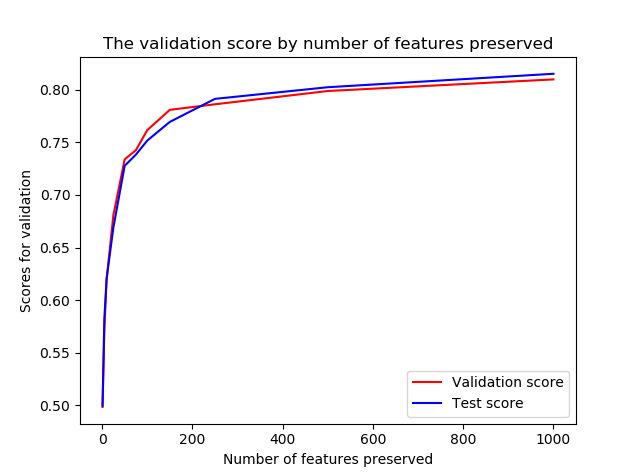
\includegraphics[width=0.7\textwidth]{Val_Test_Scores.png}
		\caption{The average validation and test scores after averaging the scores for the data sets and ranking methods.}
		\label{fig:ValTestScores}
	\end{figure}
	
	% Discussion result validation and test scores
	As could be seen (Figure \ref{fig:ValTestScores}) the difference between the validation and the test scores was very low. The average almost showed two identical curves which indicates that there was hardly any overfitting present for filter methods. The test error should not be higher than the validation error usually, but in this case the test error had a higher variance. The test error was only one measurement (after splitting the data into training and test set) and the validation error was found with leave-one-out, which should have a much lower variance. Because of the lower variance, the validation score was used in the other two figures (Figures \ref{fig:MachineLearningQualityScores} and \ref{fig:DatasetRankScores}).
	
	% Insert figures
	\begin{figure}[H]
		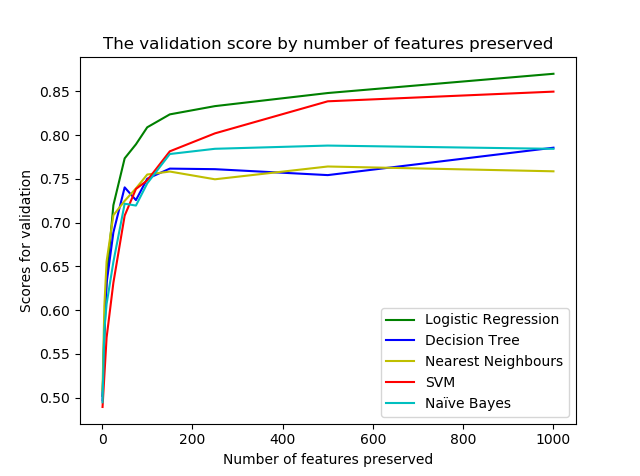
\includegraphics[width=0.7\textwidth]{Machine_Learning_Val_Scores.png}
		\caption{The average validation scores shown per machine learning quality measurement.}
		\label{fig:MachineLearningQualityScores}
	\end{figure}

	% Discussion machine learning quality scores
	Logistic regression gave the best validation scores taking all data sets combined, followed by SVM. Also, when looking at all eight plots separately (Appendix \ref{app:FeatureSelectionExplorationPlots}), logistic regression also showed the most consistent behaviour. All five of the machine learning algorithms showed an 'elbow', an area in the graph for which the score stops growing as much when more features are used. This 'elbow' was located around 100 features with 200 features being the end for almost every 'elbow'.

	% Insert figures
	\begin{figure}[H]
		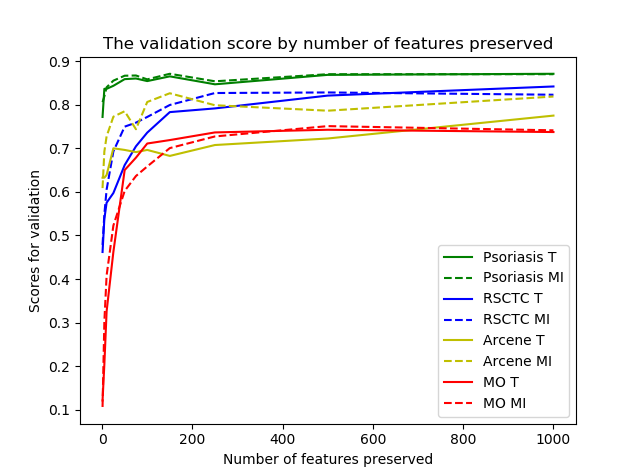
\includegraphics[width=0.7\textwidth]{Data_Rank_Val_Scores.png}
		\caption{The average validation scores shown per dataset and rank.}
		\label{fig:DatasetRankScores}
	\end{figure}
	
	% Discussion machine learning quality scores
	A difference in score quality for the datasets was visible (Figure \ref{fig:DatasetRankScores}). The difference between using Mutual Information and T-test/ANOVA was not, as for only the Arcene dataset there was a significant difference between the two. Therefore it seems that the ranking method type has less influence on the measurement quality. One interesting aspect was that methods using Mutual Information had a longer computation time than methods using the T-test/ANOVA.
	
	% Precision/Recall/F1
	Accuracy was used to test the quality of the filter methods. Aside from accuracy the precision, recall and F1-score were also computed to find out whether accuracy is a proper representation of the quality (Figure \ref{fig:DatasetRankF1Scores} and Appendix \ref{app:PrecisionRecall}). These scores showed that the accuracy is a plausible way to depict quality. Only the Arcene dataset shows some difference between accuracy, precision, recall and the F1-score but these differences would not affect any conclusions.
	
		% Insert figures
	\begin{figure}[H]
		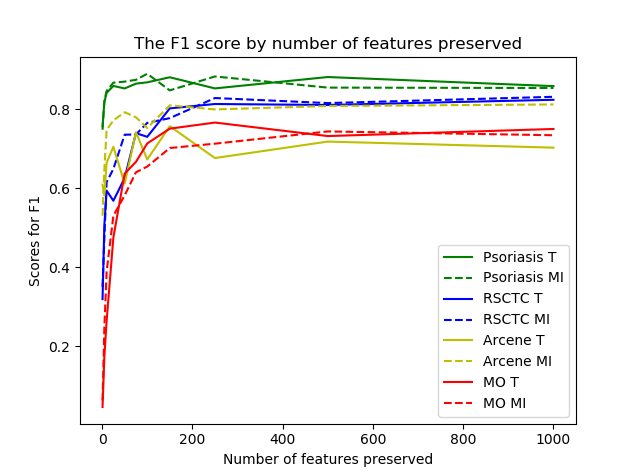
\includegraphics[width=0.7\textwidth]{Data_Rank_F1_Scores.png}
		\caption{The average F1-scores shown per dataset and rank.}
		\label{fig:DatasetRankF1Scores}
	\end{figure}
	
	\subsection{Feature Selection Algorithms Evaluation Results}
	\label{subsec:FeatureSelectionAlgorithmsEvaluationResults}
	
	% Figures + first observations
	Spectra using all basic filter methods and wrapper sequential search methods were created, averaging the accuracy (Figure \ref{fig:Avg_Accuracy_Spectrum}), precision (Figure \ref{fig:Avg_Precision_Spectrum}), recall (Figure \ref{fig:Avg_Recall_Spectrum}) and F1 score (Figure \ref{fig:Avg_F1_Spectrum}) of the four datasets. The figures showed that all wrapper algorithms preserved on average less than 61 features for these settings, whereas the performance seems to average around 75\% for all four performance scores. The filter and embedded methods performed worse, with an overall lower performance score than the wrapper methods, even when more features were present. Also, no immediate observations can be made by looking only at the filter and embedded algorithms.
	
	% Wrapper algorithms observations
	When only looking at the wrapper algorithms, some other observations could be done, as well. Ordering the features before using a wrapper method structurally gave a better result than using a random ordering. Also a threshold of $\alpha = 0.001$ usually resulted in more features and in a higher scores in comparison with a threshold of $\alpha = 0.01$. Comparing the algorithms, the floating search with ordering did best in performance, whereas the other algorithms are performing closer together.
	
	% Insert figures
	\begin{figure}[H]
		\centering
		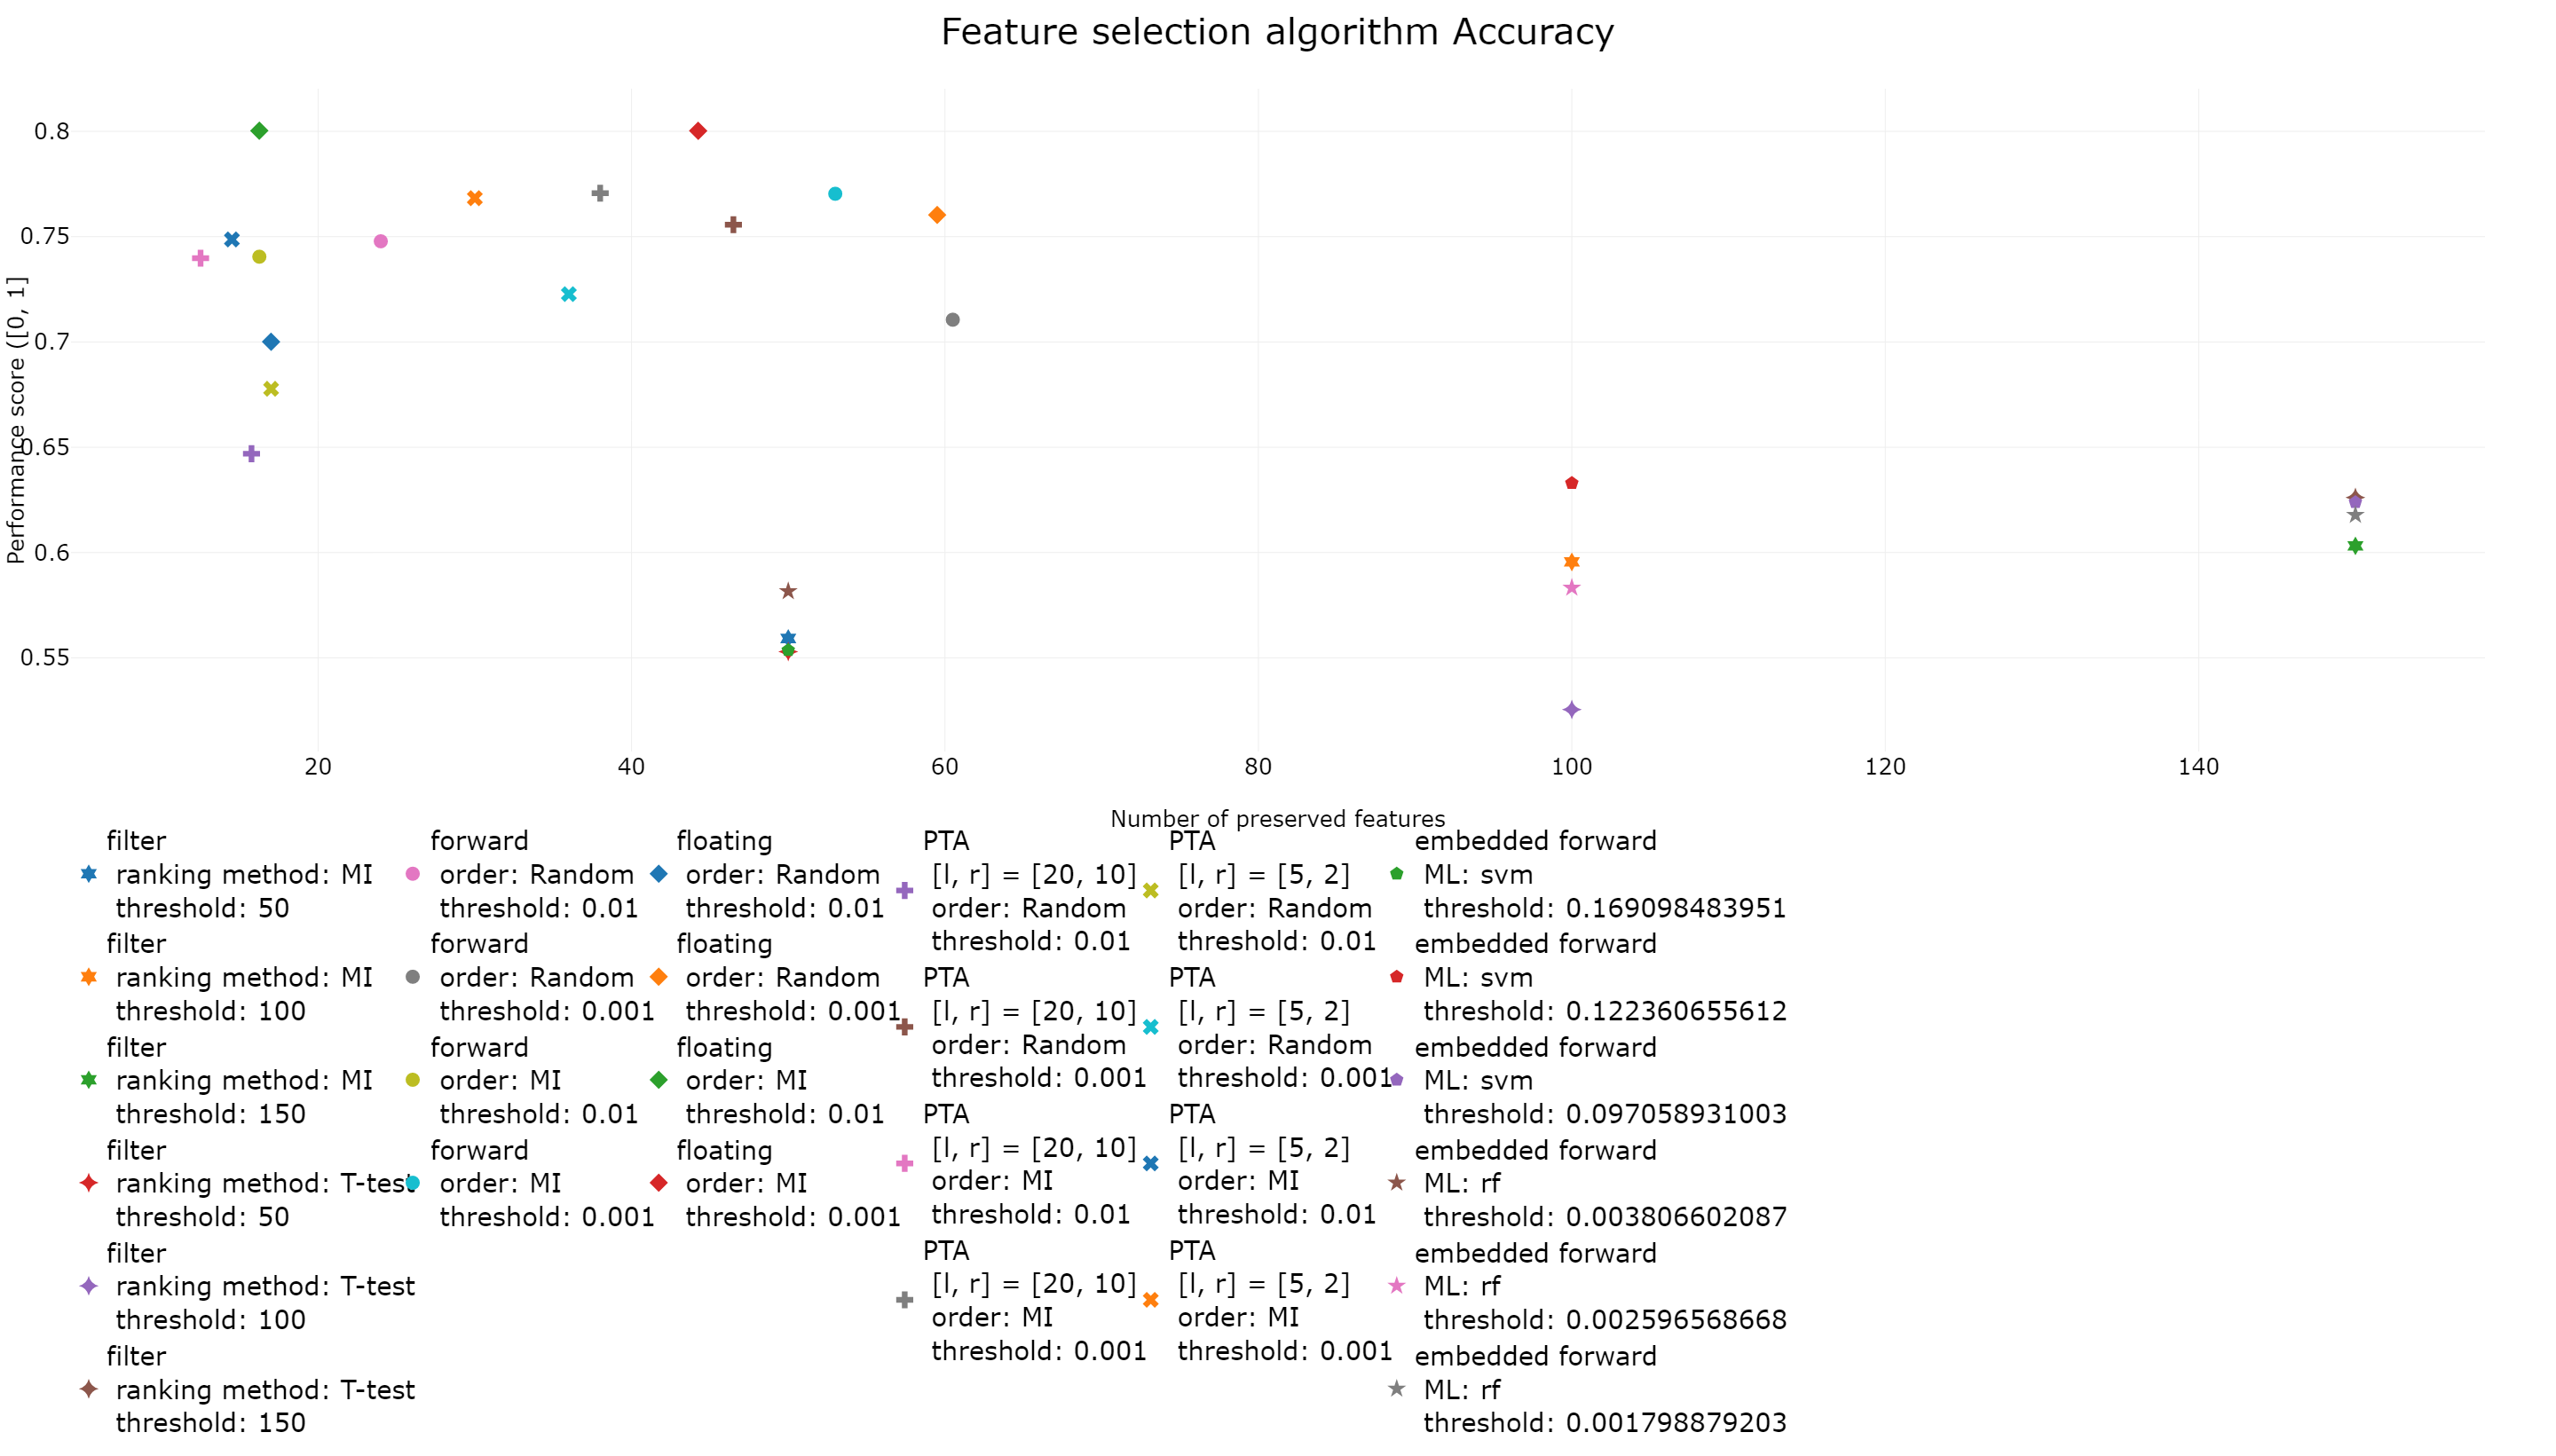
\includegraphics[angle=90,height=1.4\textwidth]{Accuracy_new.png}
		\caption{The accuracy spectrum for the average dataset. The x-axis shows the average number of features that are preserved and the y-axis shows the accuracy of logistic regression. The legend indicates the algorithms (Table \ref{tab:SecondExperimentMethods}) and their corresponding shapes, as well as the chosen parameters with their matching colours. Abbreviations in legend: Mutual Information (MI), Pick l-Take Away r (PTA), Machine Learning algorithm (ML), Support Vector Machine (svm), random forest (rf)}
		\label{fig:Avg_Accuracy_Spectrum}
	\end{figure}

	% Insert figures
\begin{figure}[H]
	\centering
	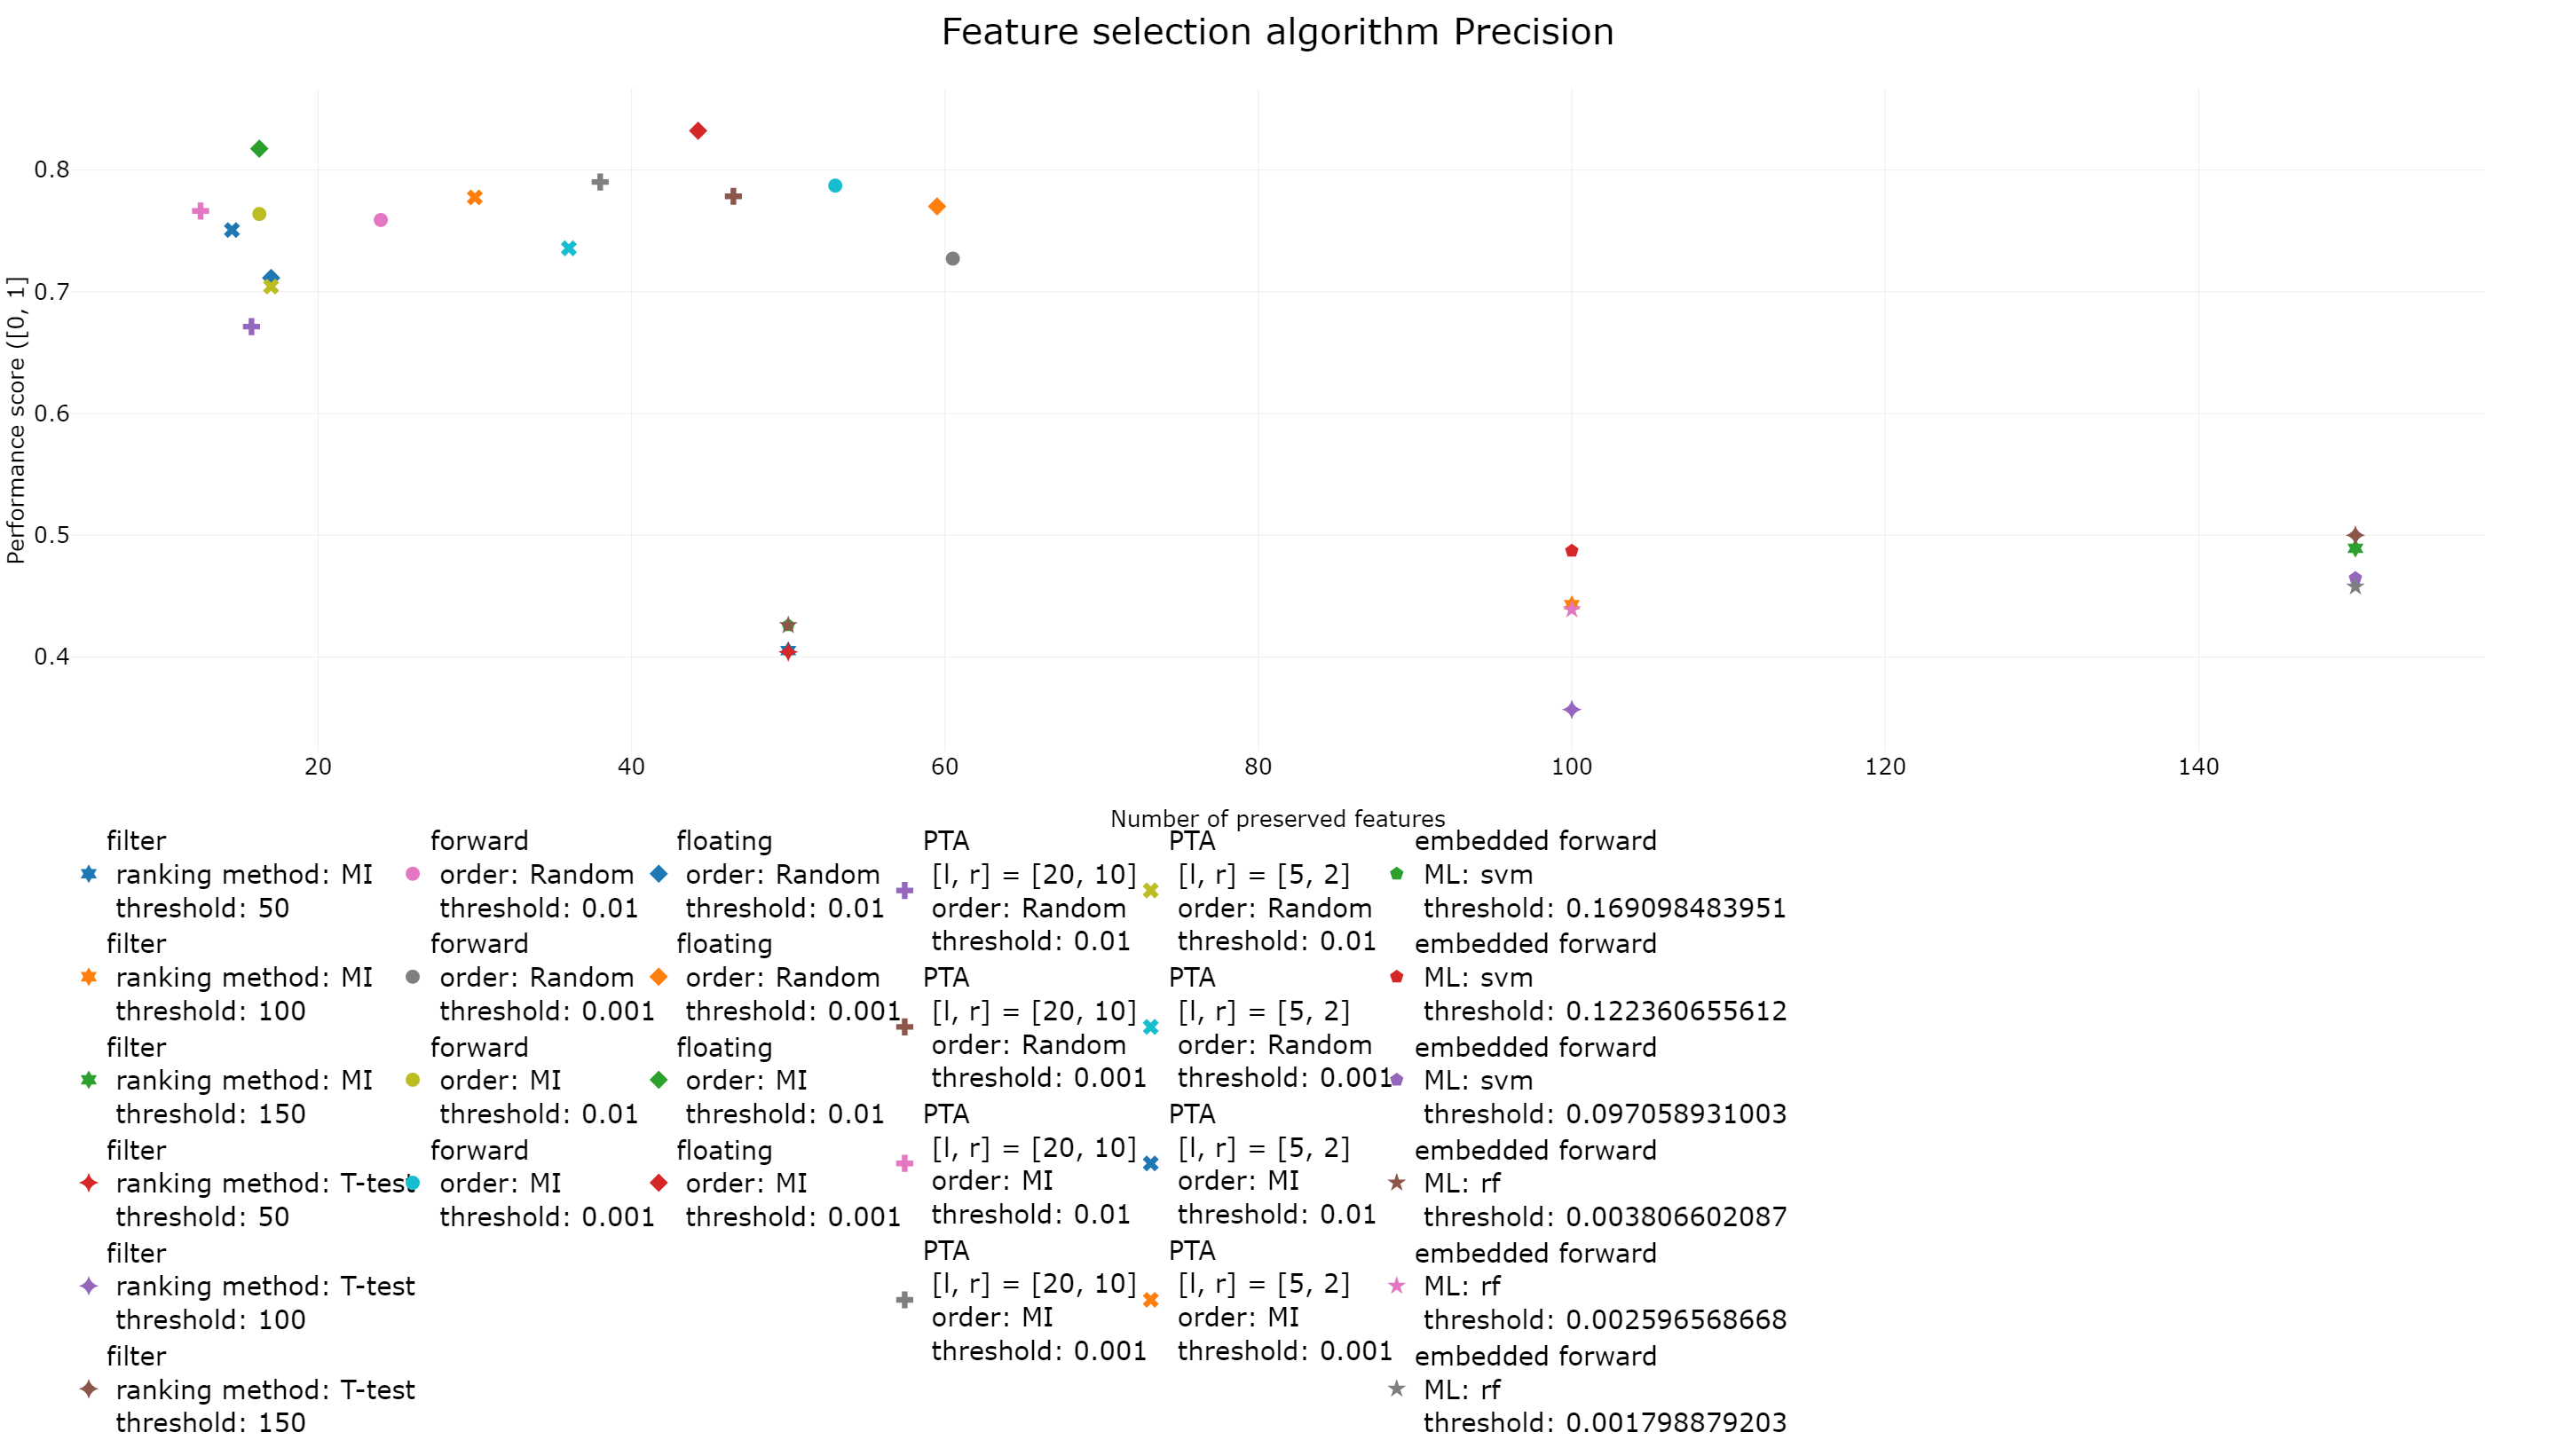
\includegraphics[angle=90,height=1.4\textwidth]{Precision_new.png}
	\caption{The precision spectrum for the average dataset. The x-axis shows the average number of features that are preserved and the y-axis shows the precision of logistic regression. The legend indicates the algorithms and their corresponding shapes, as well as the chosen parameters with their matching colours. Abbreviations in legend: Mutual Information (MI), Pick l-Take Away r (PTA), Machine Learning algorithm (ML), Support Vector Machine (svm), random forest (rf)}
	\label{fig:Avg_Precision_Spectrum}
\end{figure}

	% Insert figures
\begin{figure}[H]
	\centering
	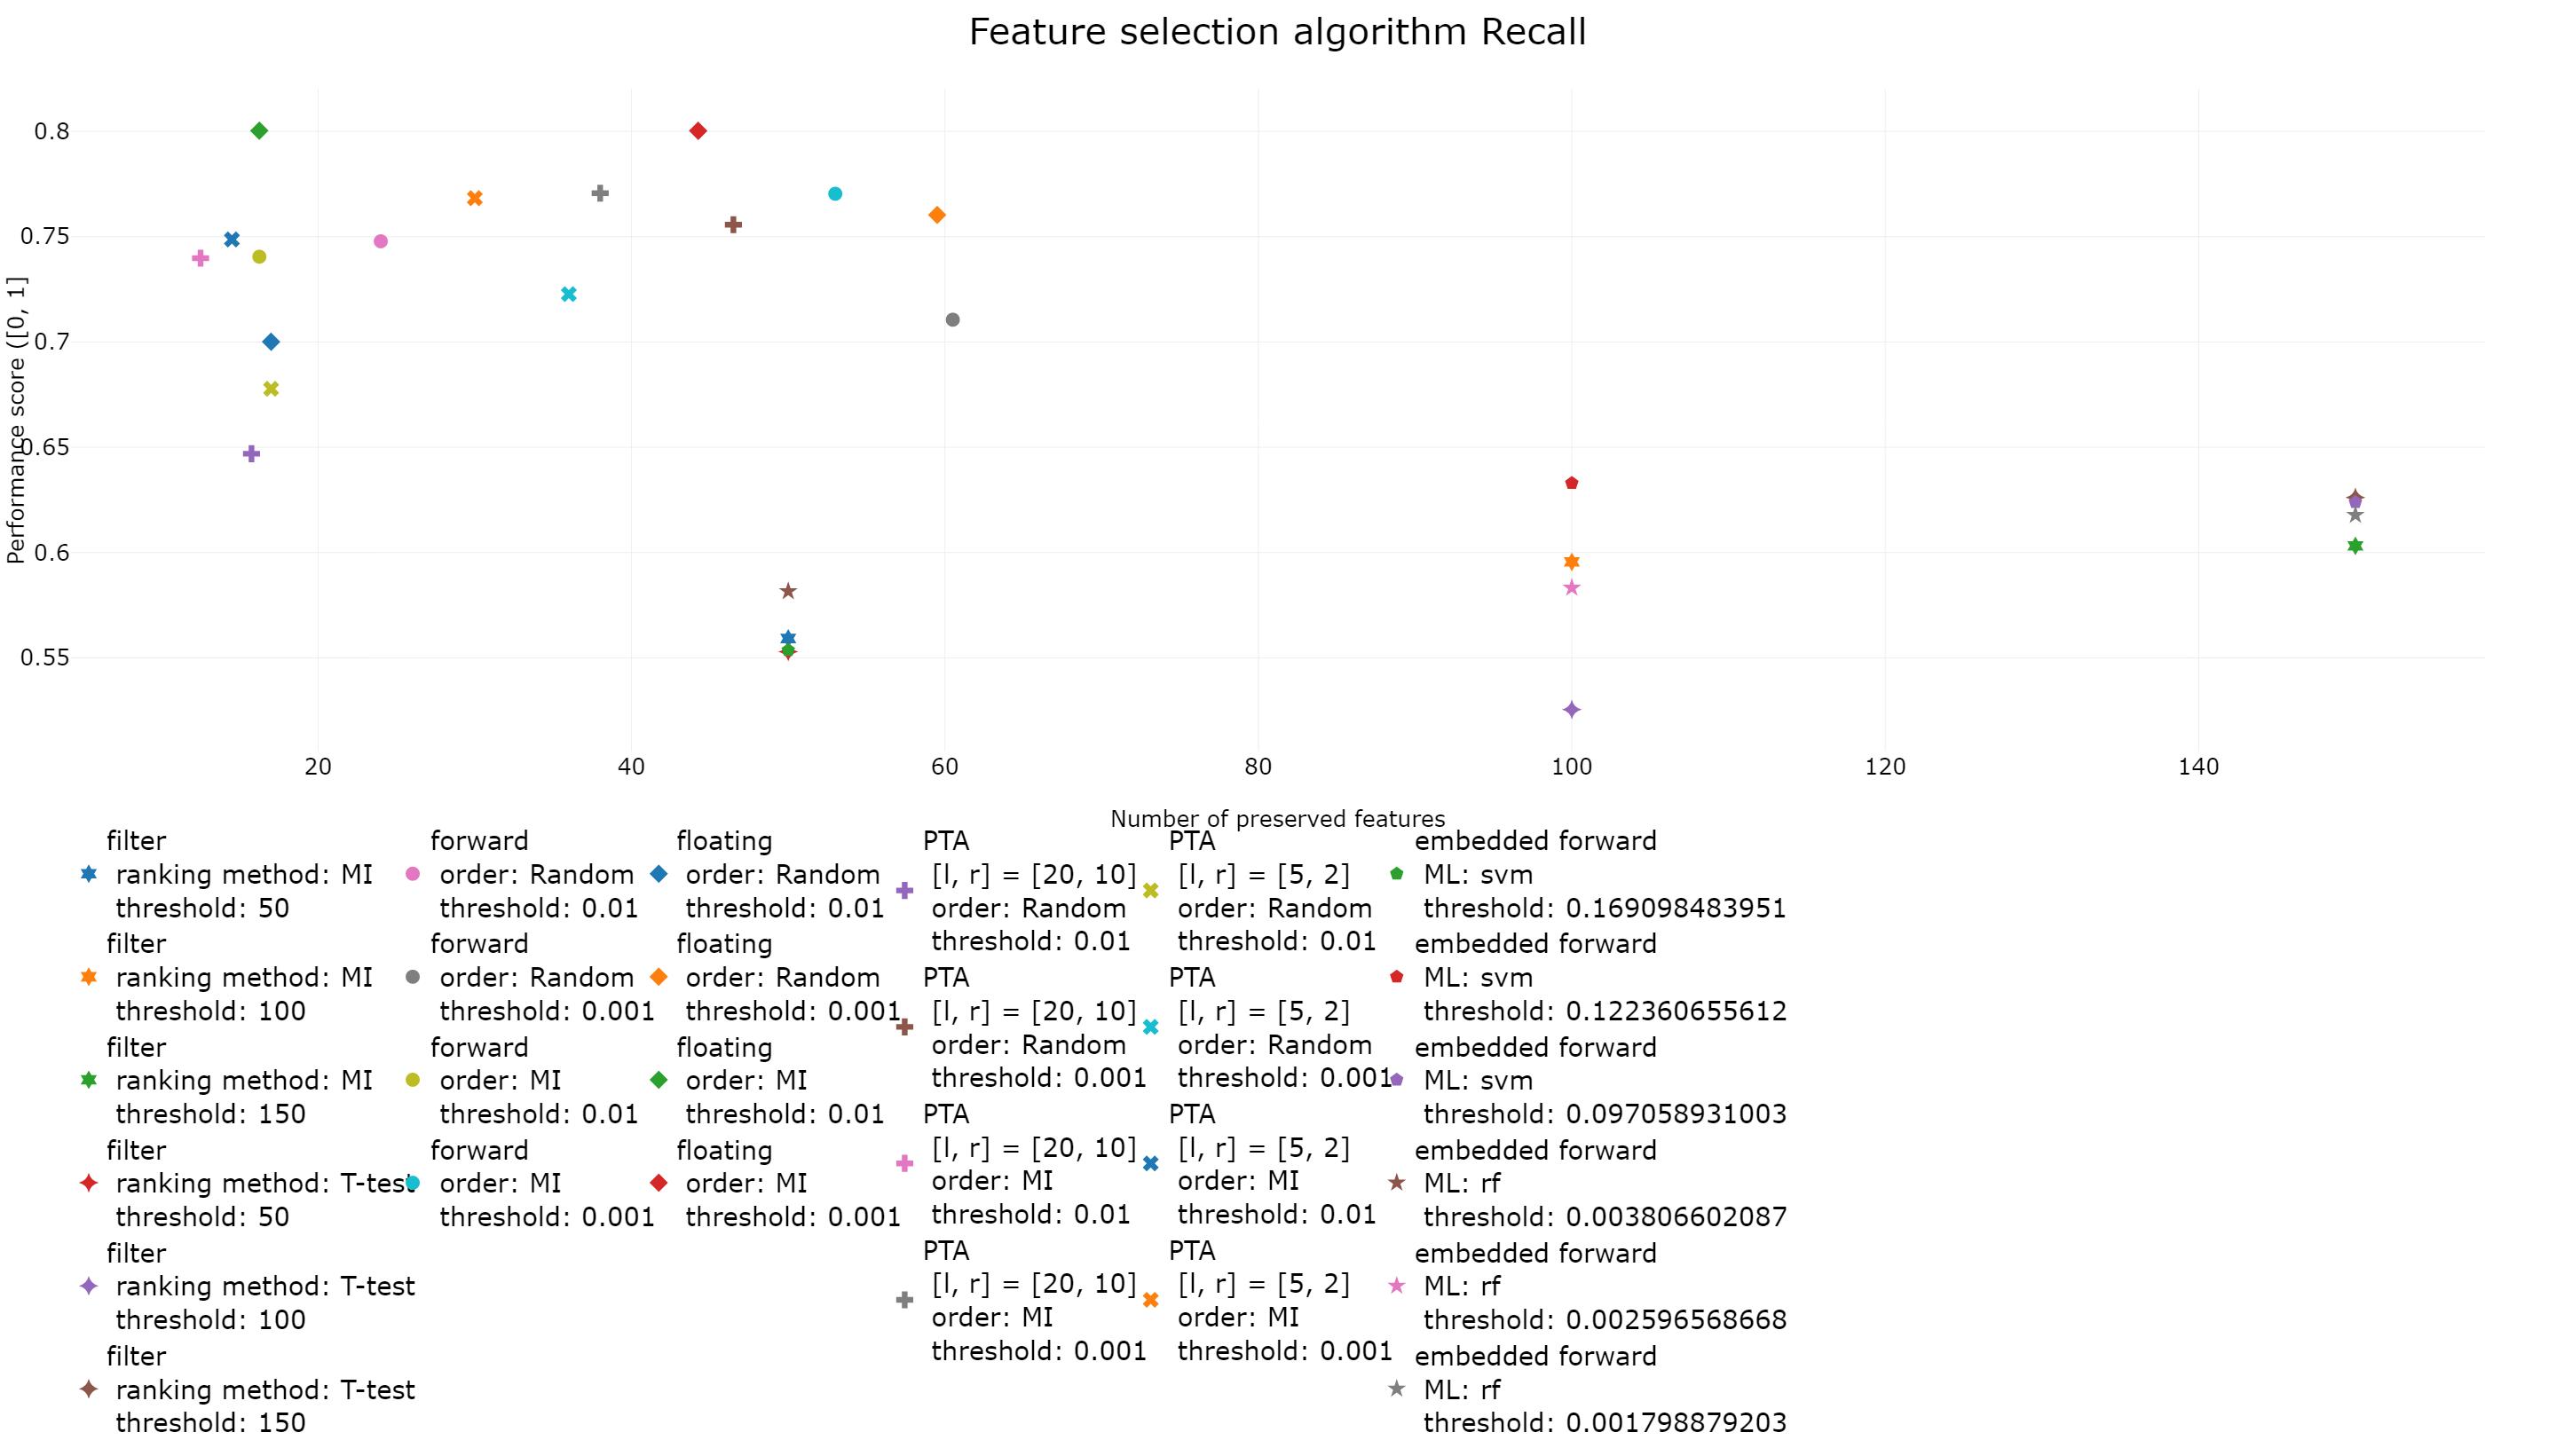
\includegraphics[angle=90,height=1.4\textwidth]{Recall_new.png}
	\caption{The recall spectrum for the average dataset. The x-axis shows the average number of features that are preserved and the y-axis shows the recall of logistic regression. The legend indicates the algorithms and their corresponding shapes, as well as the chosen parameters with their matching colours. Abbreviations in legend: Mutual Information (MI), Pick l-Take Away r (PTA), Machine Learning algorithm (ML), Support Vector Machine (svm), random forest (rf)}
	\label{fig:Avg_Recall_Spectrum}
\end{figure}

	% Insert figures
\begin{figure}[H]
	\centering
	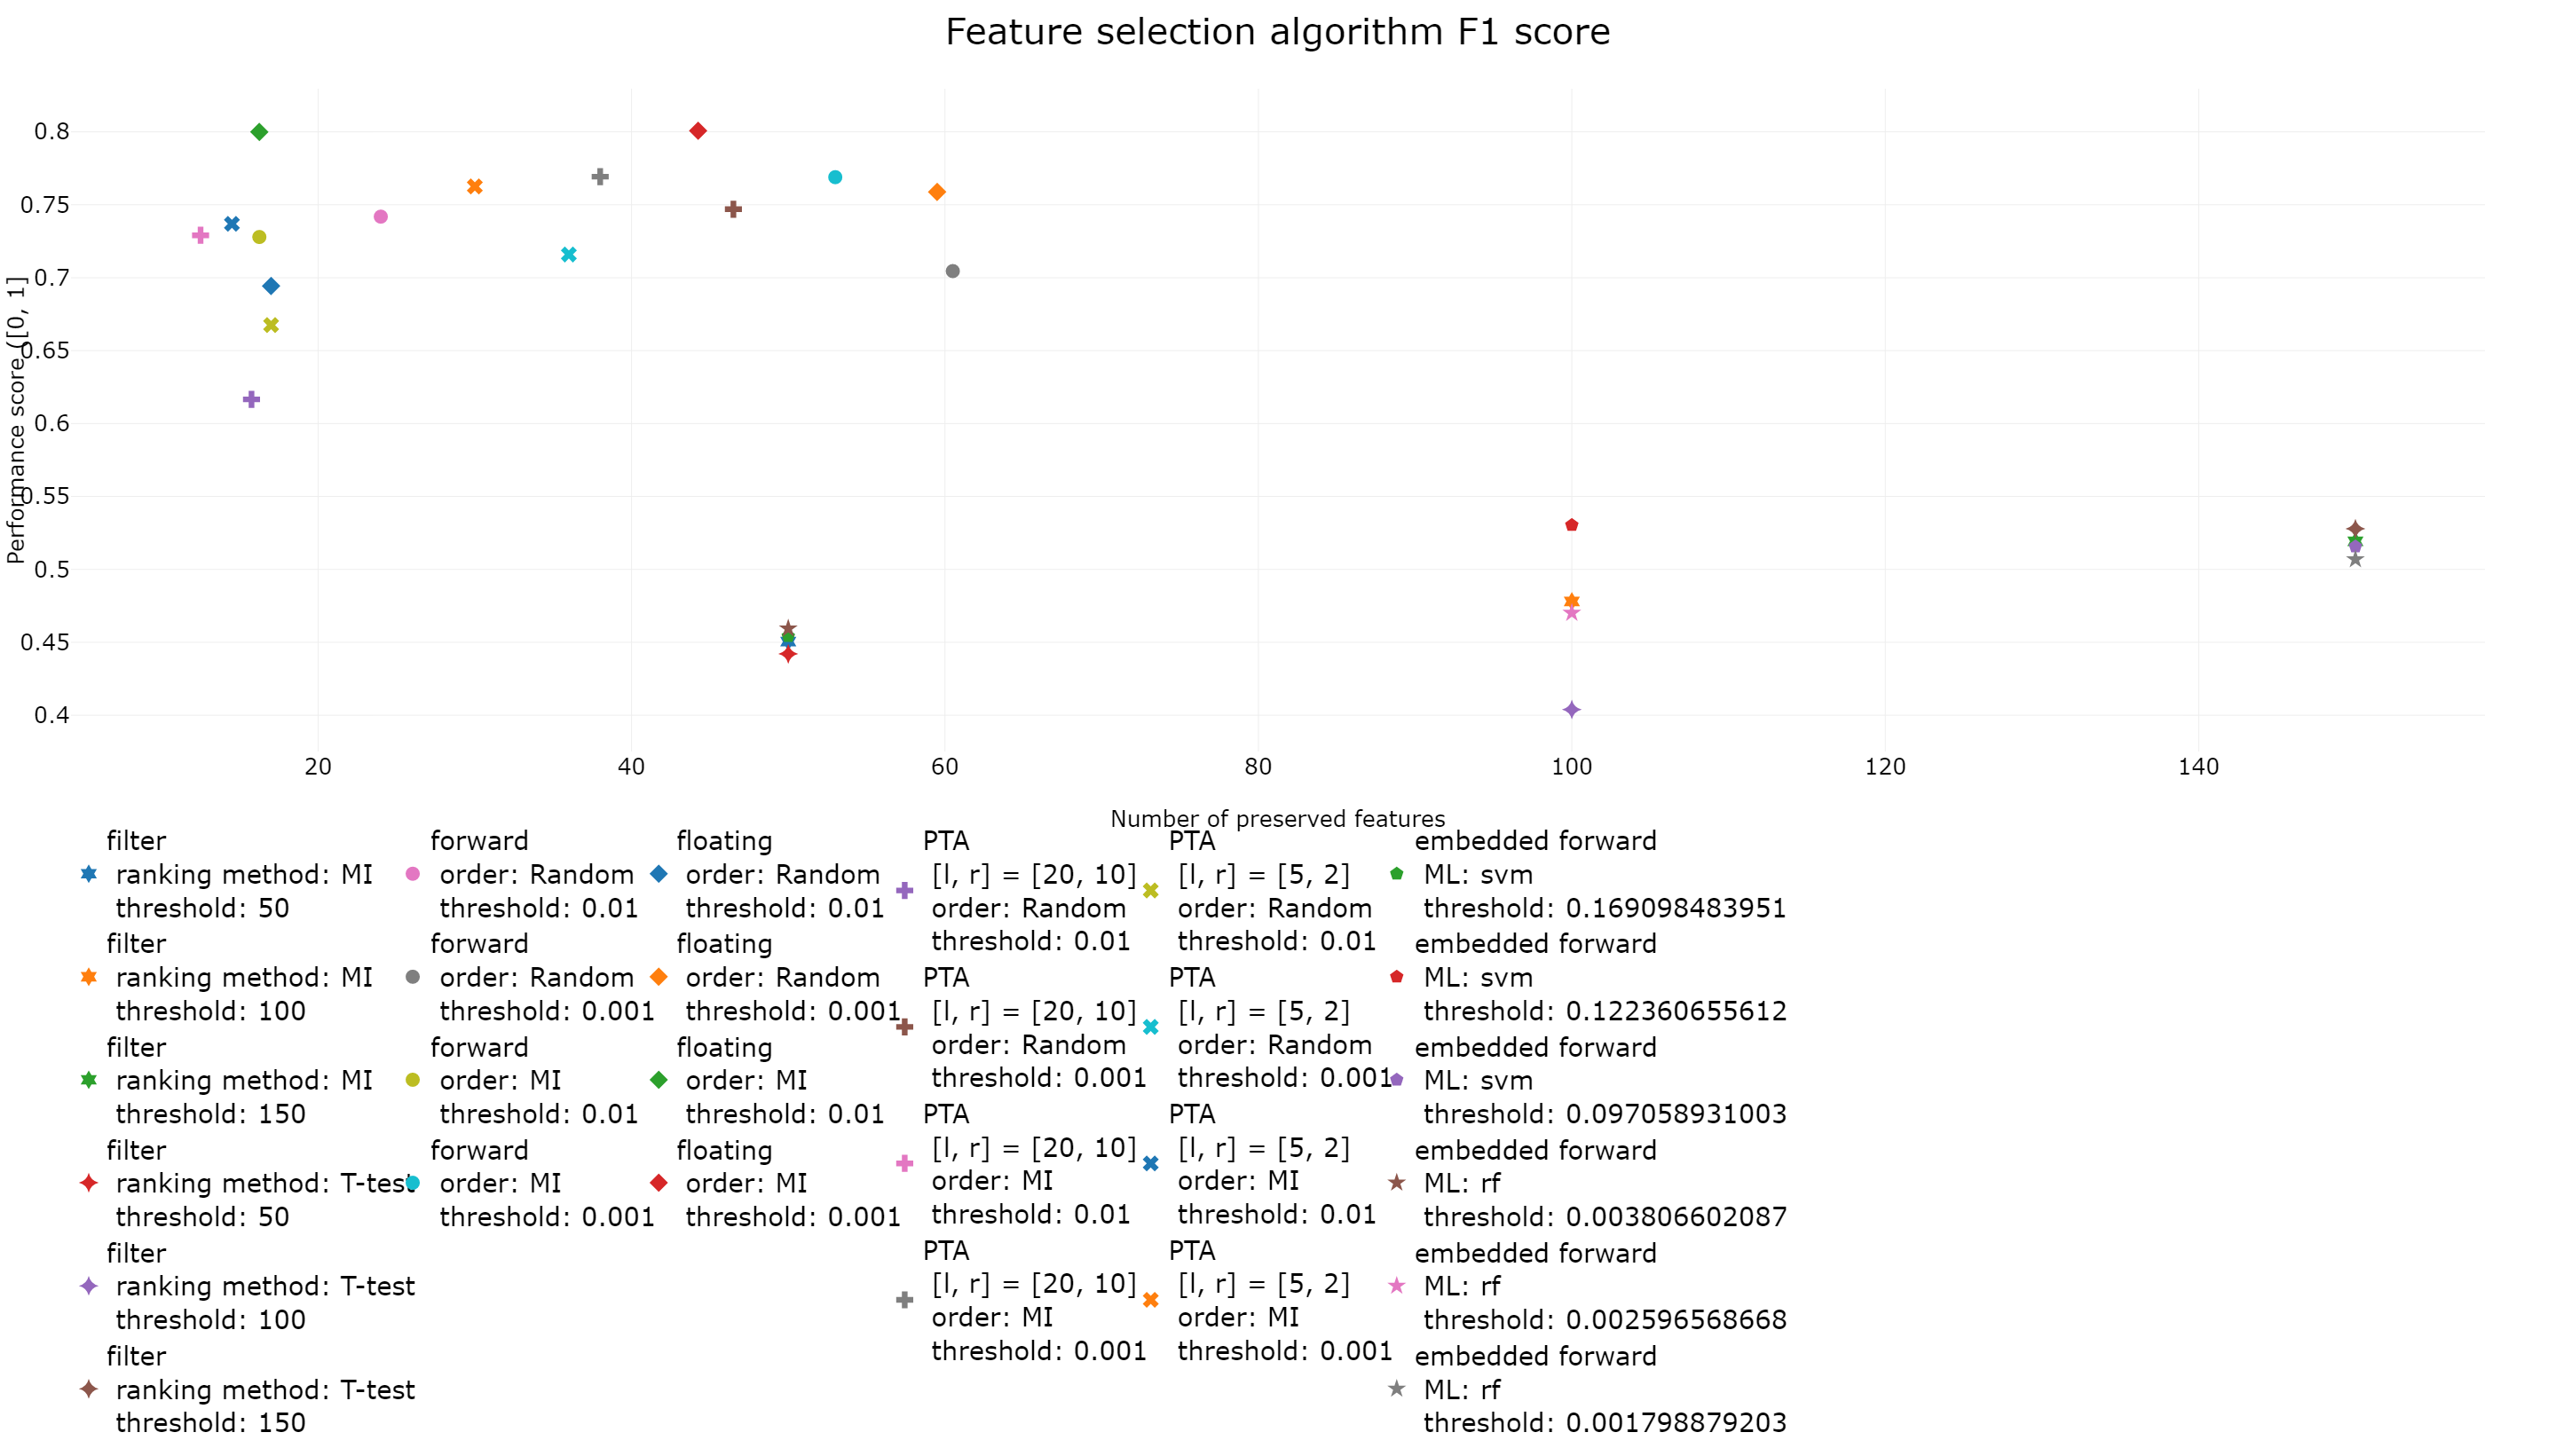
\includegraphics[angle=90,height=1.4\textwidth]{F1_new.png}
	\caption{The F1 spectrum for the average dataset. The x-axis shows the average number of features that are preserved and the y-axis shows the F1 score of logistic regression. The legend indicates the algorithms and their corresponding shapes, as well as the chosen parameters with their matching colours. Abbreviations in legend: Mutual Information (MI), Pick l-Take Away r (PTA), Machine Learning algorithm (ML), Support Vector Machine (svm), random forest (rf)}
	\label{fig:Avg_F1_Spectrum}
\end{figure}

	% Computation time
	Aside from the ability to preserve the correct features, also an evaluation of the computation time was made for the different algorithms (Figure \ref{fig:Comp_Time_Bar}). This chart immediately showed that the wrapper methods took significantly more computation time, with floating search to be take the longest. There was no major difference between forward selection and both PTA's, however there was a difference between filter methods using Mutual Information and T-test. Also for the embedded methods, the SVM based embedded method took significantly less time as well, compared with the random forest embedded method.

	% Insert figures
\begin{figure}[H]
	\centering
	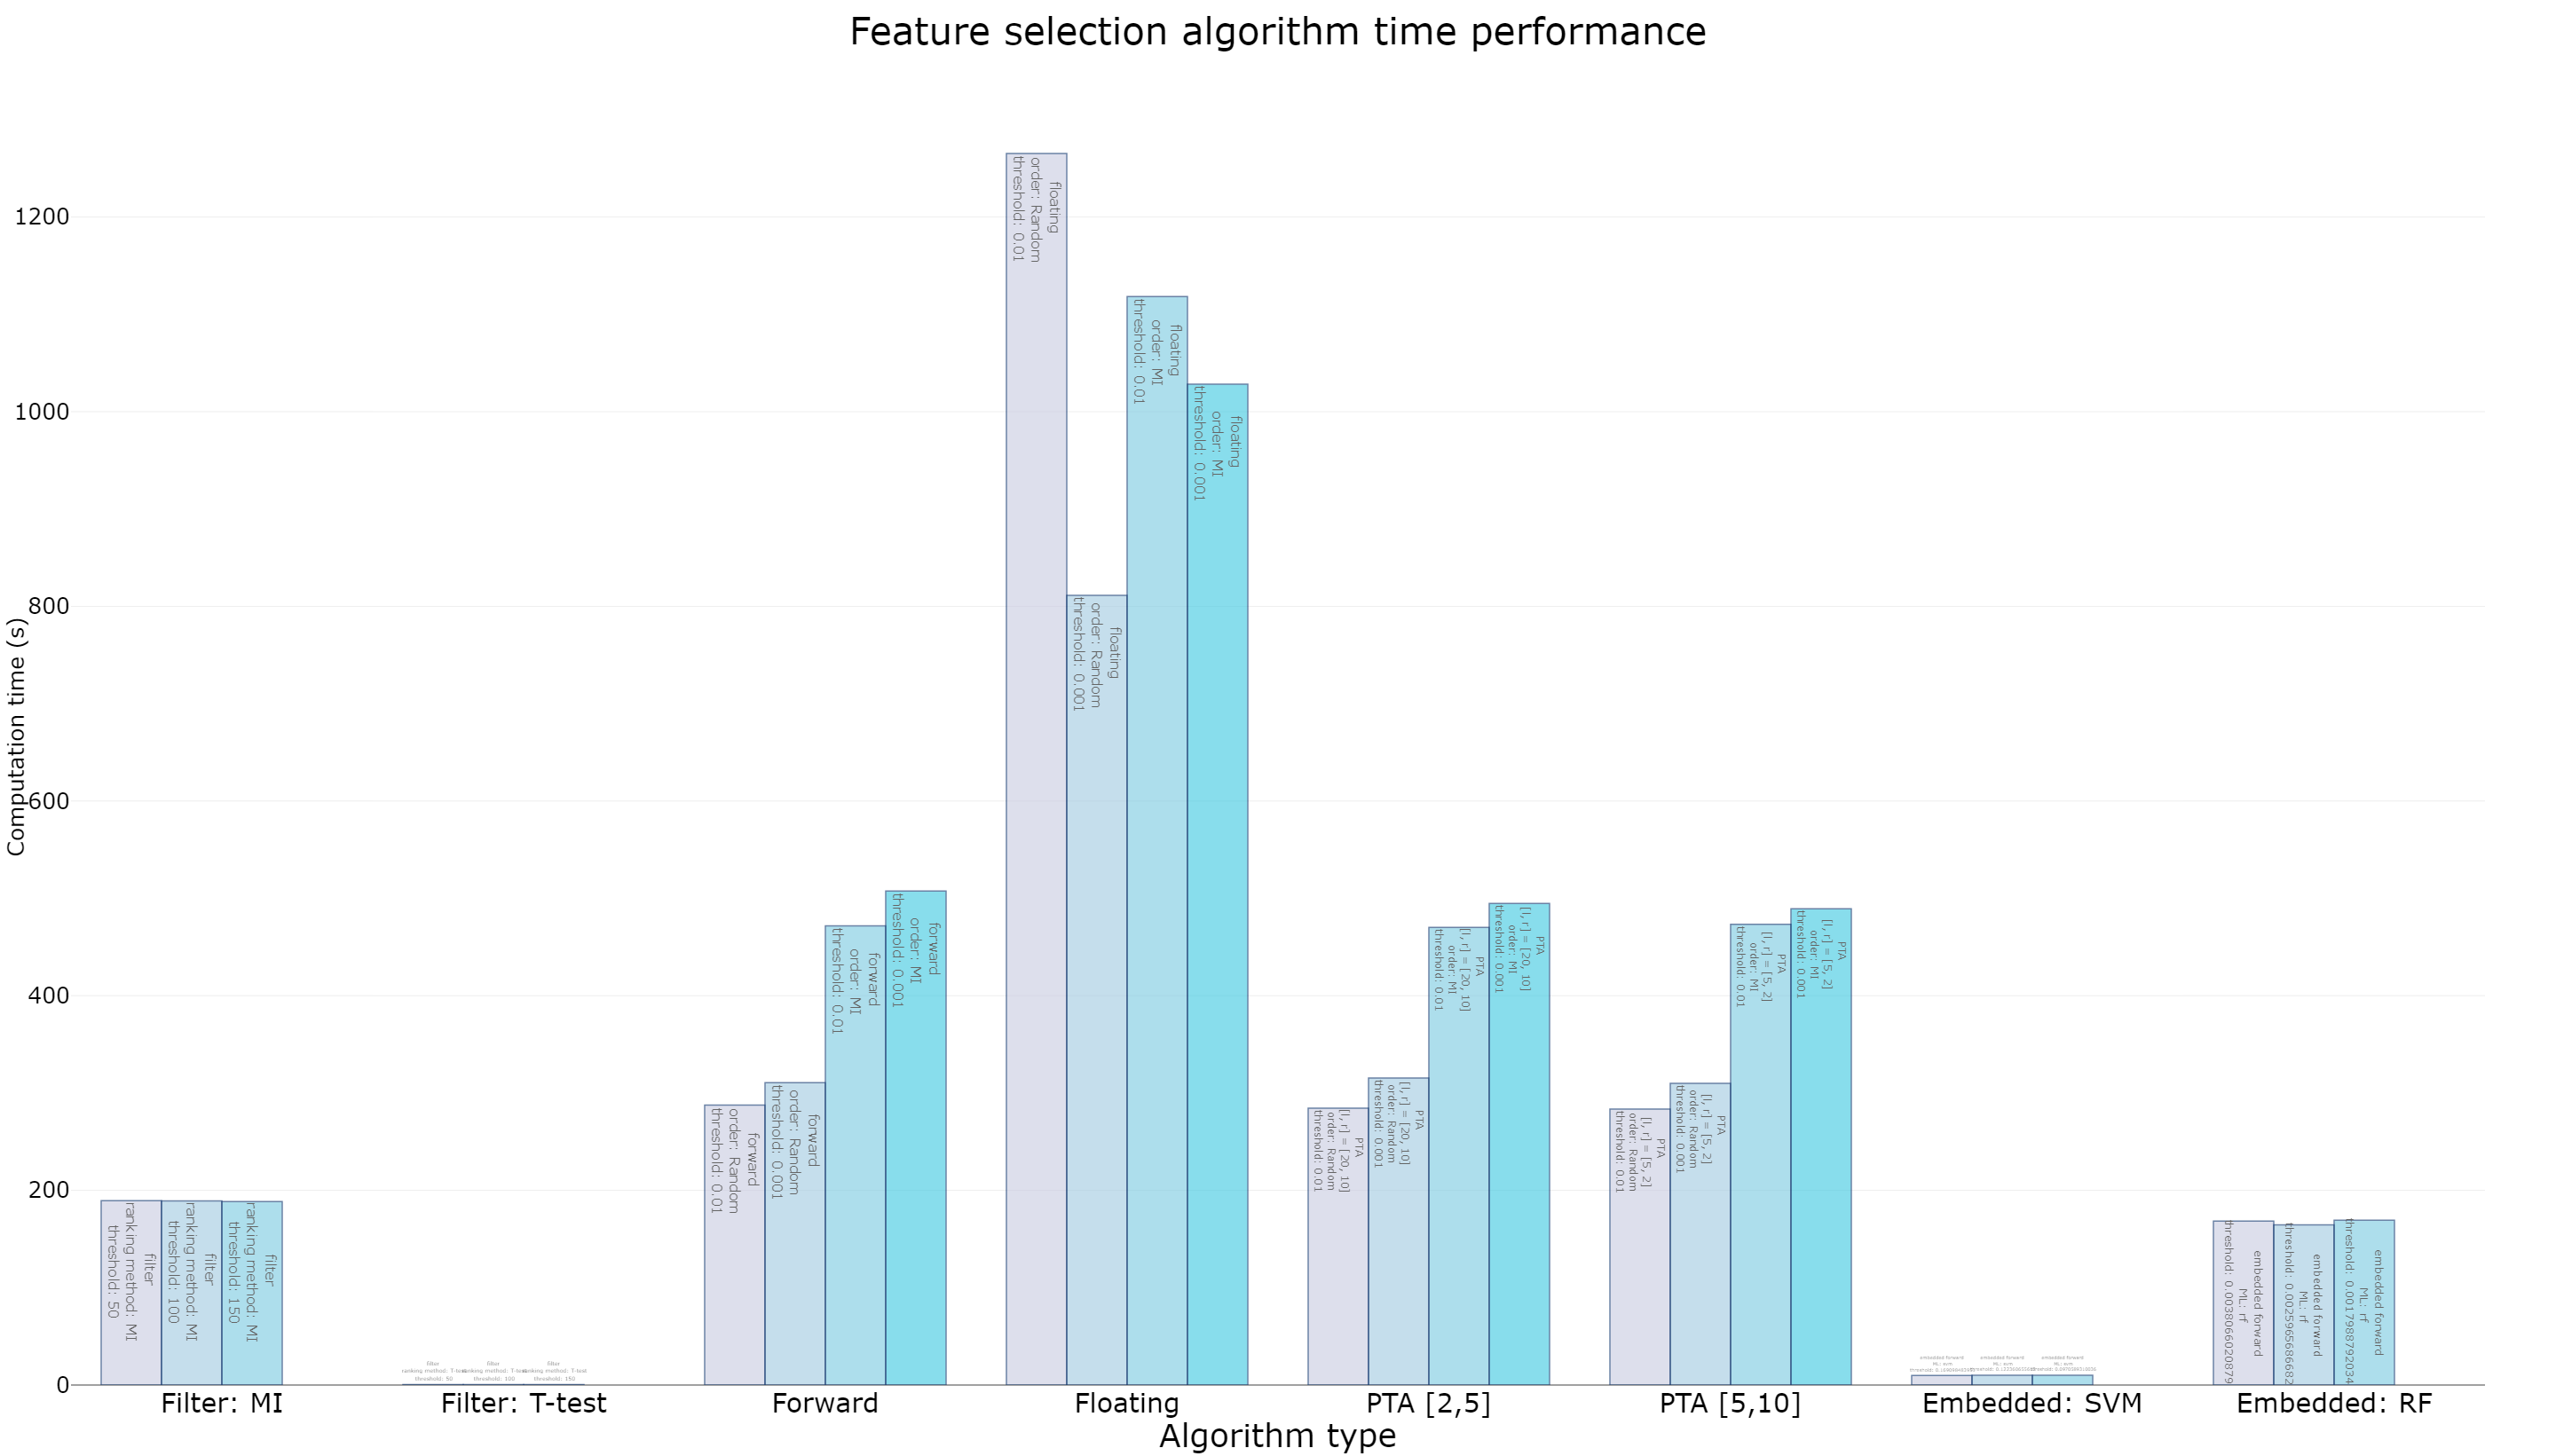
\includegraphics[angle=90,height=1.4\textwidth]{ComputationTimeBarChart.png}
	\caption{A bar chart showing the average computation time of all evaluated algorithms. The x-axis corresponded to the different algorithms, for which the computation time for multiple parameter combinations were given. The y-axis corresponded to the computation time in seconds. Abbreviations in legend: Mutual Information (MI), Pick l-Take Away r (PTA), Support Vector Machine (svm), random forest (rf)}
	\label{fig:Comp_Time_Bar}
\end{figure}

	% FS_Accuracy
	At last the relation between the computation time and FS\_accuracy, the corrected accuracy, are visualized (Figure \ref{fig:Comp_Time_FS_Acc}). In this chart the trade-of between computation time and quality of a feature selection algorithm is  shown by the following statements: 
	\begin{itemize}
		\item Filter and embedded methods take the shortest time, but have the worst performance. Floating methods takes the longest time, but are not necessarily better than other wrapper methods
		\item For both filter and embedded methods using T-test and svm over mutual information and random forests respectively seems to greatly reduce computation time for little to no improvement in FS\_accuracy.
		\item For all wrapper methods the addition of an ordering and choosing a threshold of $\alpha = 0.01$ over $\alpha = 0.001$ gives better results. Using these hyper-parameters however usually add computation time.
		\item Forward selection and PTA do not show a big difference between each other.
	\end{itemize}
	
	% Insert figures
\begin{figure}[H]
	\centering
	\includegraphics[angle=90,height=1.4\textwidth]{FS_Accuracy_99.png}
	\caption{The relation between the FS\_accuracy and the computation time. The x-axis shows the computation time the y-axis shows the FS\_accuracy score of logistic regression. The legend indicates the algorithms and their corresponding shapes, as well as the chosen parameters with their matching colours. Abbreviations in legend: Mutual Information (MI), Pick l-Take Away r (PTA), Machine Learning algorithm (ML), Support Vector Machine (svm), random forest (rf)}
	\label{fig:Comp_Time_FS_Acc}
\end{figure}
	
	\subsection{TPOT Feature Selection Integration Results}
	
	
	\begin{table}[]
		\begin{tabular}{ll|ll|ll}
			\multirow{2}{*}{\textbf{Algorithm}} & selection      & \multicolumn{2}{l|}{regular selection}                                                                                                 & \multicolumn{2}{l}{always feature selection}                                               \\ \cline{3-6} 
			& availability   & \begin{tabular}[c]{@{}l@{}}regular\\ algorithms\end{tabular} & \begin{tabular}[c]{@{}l@{}}feature selection\\ algorithms\end{tabular} & regular algorithms & \begin{tabular}[c]{@{}l@{}}feature selection\\ algorithms\end{tabular} \\ \hline
			\multirow{4}{*}{\textbf{Datasets}}  & MicroOrganisms & 0.79                                                        & 0.65                                                                  & 0.89               & 0.85                                                                   \\
			& Arcene         & 0.89                                                        & 0.89                                                                  & 0.88               & 0.84                                                                   \\
			& RSCTC          & 0                                                       & 0.55                                                                 & 0.91               & 0.60                                                                       \\
			& Psoriasis      & 0.78                                                       & 0.77                                                                 & 0.91                   & 0.72                                                                      
		\end{tabular}
	\end{table}
	
	\newpage
	\section{Discussion}
	\label{sec:Discussion}
	
	% Research relevance
	Several scientist researched the possibility of feature selection, both with a data analytical\cite{catal2009investigating} as well as a biomedical\cite{baumgartner2006data, welthagen2005comprehensive, liu2002comparative} point of view. These research projects usually focused on datasets with a low number of features, for which feature selection is less relevant. Doing research for datasets that have a significantly higher number of at least 1000 features is new, even though newly available datasets become bigger over time due to new and improved techniques of measuring and storing data. With this research a beginning is made on how to approach feature selection on these bigger datasets.
	
	% Wrapper methods exclusion
	Whereas multiple feature selection methods are discussed, several were not tested due to computation time constraints. The wrapper methods backwards elimination and simulated annealing and the embedded backwards elimination all were too computationally intensive to become relevant for the research. In datasets with fewer features, these methods may be showing better results and could be possible candidates for feature selection.
	
	
	\section{Conclusions}	
	\label{sec:Conclusions}
	
	% Filter method exploration
	After evaluation of the results in the first experiment set-up, it can be concluded that there is not a big difference between using T-test/ANOVA or Mutual Information as a ranking method. Both seem to give similar results, with the exception of one dataset (Figure \ref{fig:DatasetRankScores}). The T-test/ANOVA is computationally faster than Mutual Information as could be seen in the second experiment (Figure \ref{fig:Comp_Time_Bar}), however also works with the assumption that the classes are normally distributed. This may not always be the case. A rule of thumb for choice of ranking method would be to use t-test, except for when the data is not normally distributed. Both of them should definitely be considered to be used in the framework.
	
	% Second conclusion exploration
	A second conclusion can be drawn from looking at the accuracy with the number of features preserved. After a threshold of 200 features, additional features do not raise the validation score as much as the first 200 features seem to do. This can indicate a second rule of thumb, that at least 200 features must be preserved after using a filter method. This rule of thumb is according to the hypothesized notion that at most 1000 features should be preserved to still show an efficient result, however is much lower than the expected than the upper bound.
	
	% Second experiment - filter vs wrapper methods
	After evaluation of both filter, wrapper and embedded methods, wrapper methods seem to be significantly better at selecting a smaller fraction of features while preserving a similar test score.  Whereas the expectation was for wrapper methods to be best in efficiency, embedded methods were expected to outperform both filter methods and wrapper methods when looking at both quality and computation time. This is not the case however as embedded methods had a near identical quality to filter methods and performed much worse than wrapper methods. The outcome indicates that wrapper methods are significantly different in results and filter and embedded methods being near identical.
	
	% Further conclusions
	Since wrapper methods take dependencies between features into account, they are able to keep these dependencies at a minimum. If these dependencies are unwanted, wrapper methods seem to be more useful than filter methods and embedded and should be recommended. A downside of the wrapper methods however is that they take much more computation time than the filter methods and embedded. Therefore if it does not matter if features have dependencies with each other, a filter method should be recommended.
	
	% Wrapper methods with each other
	There is a difference in quality within the wrapper methods. The forward selection and PTA all showed promising results and therefore should be considered for the framework. Floating search showed the best results, however took significantly longer in computation time. Within the wrapper methods, an ordering beforehand is recommended for improved results. Backward elimination wrapper algorithms, stochastic search algorithms and embedded backwards elimination algorithms all were significantly worse in computation time than the other wrapper algorithms and therefore should not be considered in these cases.
	
	% Threshold wrapper methods
	A recommendation for the threshold in wrapper methods is not trivial. A higher threshold of $\alpha = 0.01$ gives a smaller feature subset at the cost of a lower classification score. If a smaller subset is desired of high influence features is needed, a bigger threshold should be chosen, whereas it will be smaller if the quality of the feature subset is better.
	
	% Combinations
	In this research only separate feature selection methods were tested. Whereas the filter methods needed very little computation time, the feature subset size and quality of the wrapper methods are much more interesting for further research. A combination of a filter and a wrapper method might create a better result. If first the majority of the features is filtered out by a filter method and then a wrapper method computes the best combination of feature, the result could be relatively quicker than the wrapper method while still maintaining a high enough quality. This combination is worth investigating into in future research.
	
	% TPOT conclusion
	% Inser here
	
	\bibliography{../References/Citings} 
	\bibliographystyle{ieeetr}
	
	\appendix
	
	\section{Feature Selection Exploration Plots}
	\label{app:FeatureSelectionExplorationPlots}
	
	The validation and test score for all combinations of dataset, ranking method and machine learning quality measure (Table \ref{tab:FirstExperimentRequirements}) in figures (Figures \ref{fig:MO_MI_Val_Test_Score}, \ref{fig:MO_T_Val_Test_Score}, \ref{fig:Arcene_MI_Val_Test_Score}, \ref{fig:Arcene_T_Val_Test_Score}, \ref{fig:RSCTC_MI_Val_Test_Score}, \ref{fig:RSCTC_T_Val_Test_Score}, \ref{fig:Psoriasis_MI_Val_Test_Score} and \ref{fig:Psoriasis_T_Val_Test_Score}). 
	
	% Insert figures
	\begin{figure}[H]
		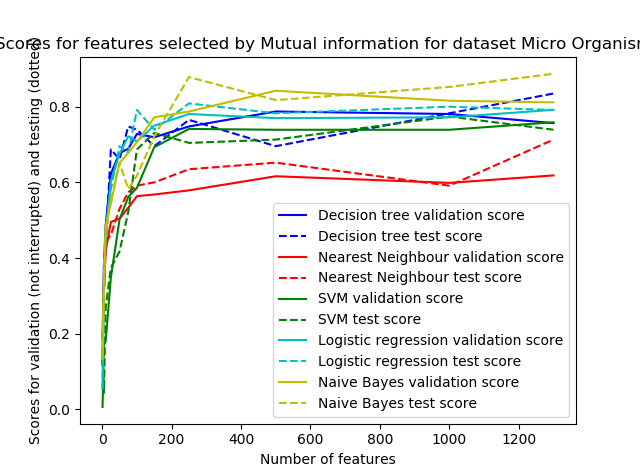
\includegraphics[width=0.7\textwidth]{MO_MI_Val_Test_Score.png}
		\caption{The validation and test score per feature preserved for the micro organisms data set with ranking method mutual information. Five different classification algorithms are used to define this classification and test score.}
		\label{fig:MO_MI_Val_Test_Score}
	\end{figure}
	
	% Insert figures
	\begin{figure}[H]
		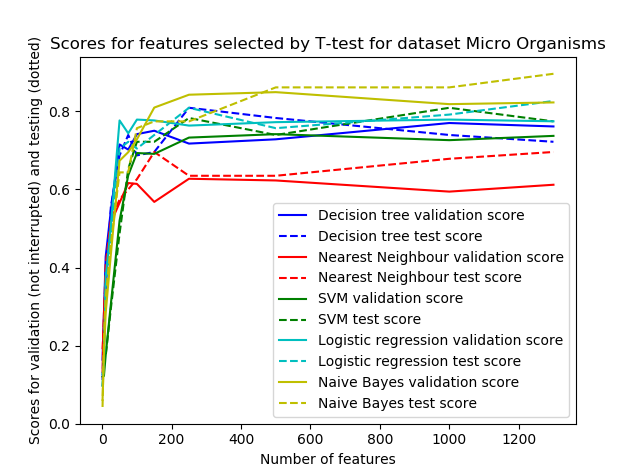
\includegraphics[width=0.7\textwidth]{MO_T_Val_Test_Score.png}
		\caption{The validation and test score per feature preserved for the micro organisms dataset with ranking method T-test. Five different classification algorithms are used to define this classification and test score.}
		\label{fig:MO_T_Val_Test_Score}
	\end{figure}

	% Insert figures
	\begin{figure}[H]
		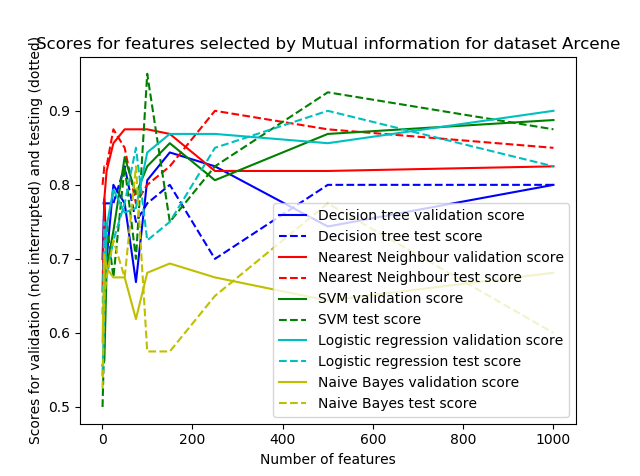
\includegraphics[width=0.7\textwidth]{Arcene_MI_Val_Test_Score.png}
		\caption{The validation and test score per feature preserved for the Arcene dataset with ranking method mutual information. Five different classification algorithms are used to define this classification and test score.}
		\label{fig:Arcene_MI_Val_Test_Score}
	\end{figure}

	% Insert figures
	\begin{figure}[H]
		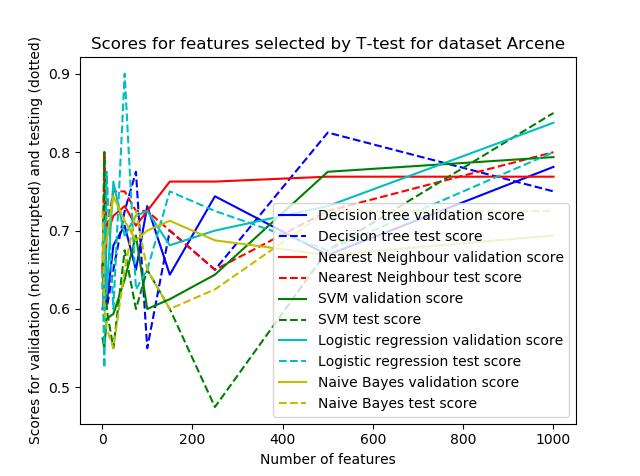
\includegraphics[width=0.7\textwidth]{Arcene_T_Val_Test_Score.png}
		\caption{The validation and test score per feature preserved for the Arcene dataset with ranking method T-test. Five different classification algorithms are used to define this classification and test score.}
		\label{fig:Arcene_T_Val_Test_Score}
	\end{figure}

	% Insert figures
	\begin{figure}[H]
		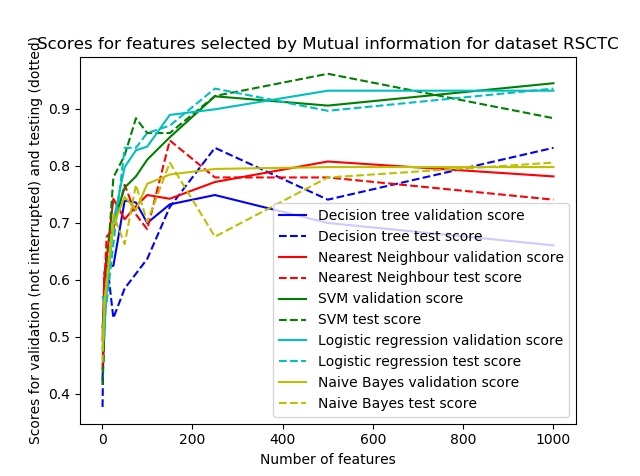
\includegraphics[width=0.7\textwidth]{RSCTC_MI_Val_Test_Score.png}
		\caption{The validation and test score per feature preserved for the RSCTC dataset with ranking method mutual information. Five different classification algorithms are used to define this classification and test score.}
		\label{fig:RSCTC_MI_Val_Test_Score}
	\end{figure}

	% Insert figures
	\begin{figure}[H]
		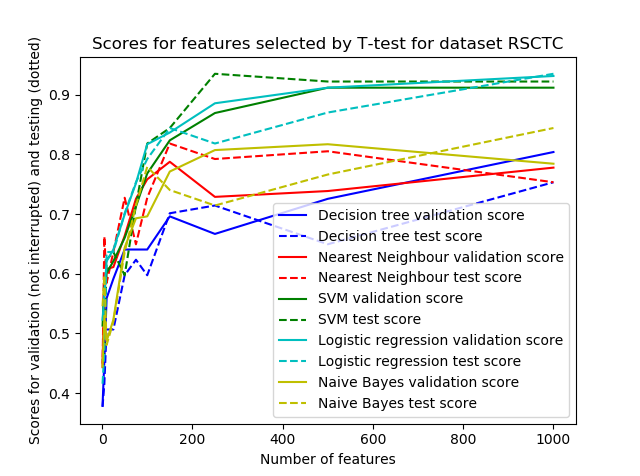
\includegraphics[width=0.7\textwidth]{RSCTC_T_Val_Test_Score.png}
		\caption{The validation and test score per feature preserved for the RSCTC dataset with ranking method T-test. Five different classification algorithms are used to define this classification and test score.}
		\label{fig:RSCTC_T_Val_Test_Score}
	\end{figure}
	
	% Insert figures
	\begin{figure}[H]
		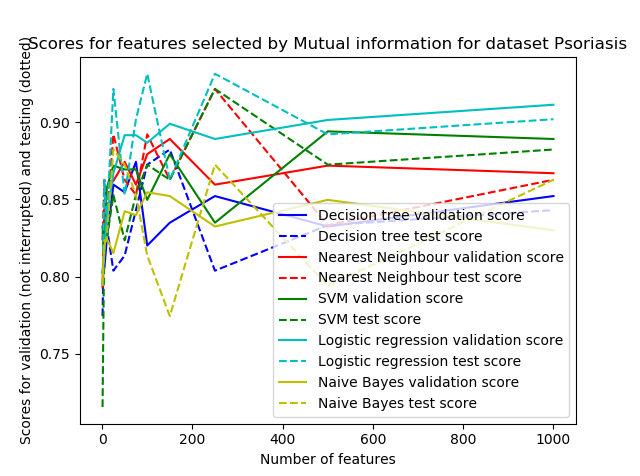
\includegraphics[width=0.7\textwidth]{Psoriasis_MI_Val_Test_Score.png}
		\caption{The validation and test score per feature preserved for the Psoriasis dataset with ranking method mutual information. Five different classification algorithms are used to define this classification and test score.}
		\label{fig:Psoriasis_MI_Val_Test_Score}
	\end{figure}
	
	% Insert figures
	\begin{figure}[H]
		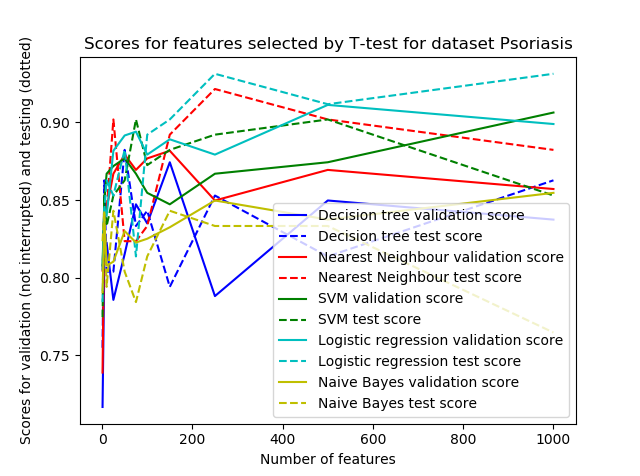
\includegraphics[width=0.7\textwidth]{Psoriasis_T_Val_Test_Score.png}
		\caption{The validation and test score per feature preserved for the Psoriasis dataset with ranking method T-test. Five different classification algorithms are used to define this classification and test score.}
		\label{fig:Psoriasis_T_Val_Test_Score}
	\end{figure}
	
	\section{Feature Selection Exploration Precision And Recall}
	\label{app:PrecisionRecall}
	
	% Itnroduciton
	The average precision (Figure \ref{fig:DatasetRankPrecisionScores}) and recall (Figure \ref{fig:DatasetRankRecallScores}). These are shown per data set and per ranking method.
	
	% Insert figures
	\begin{figure}[H]
		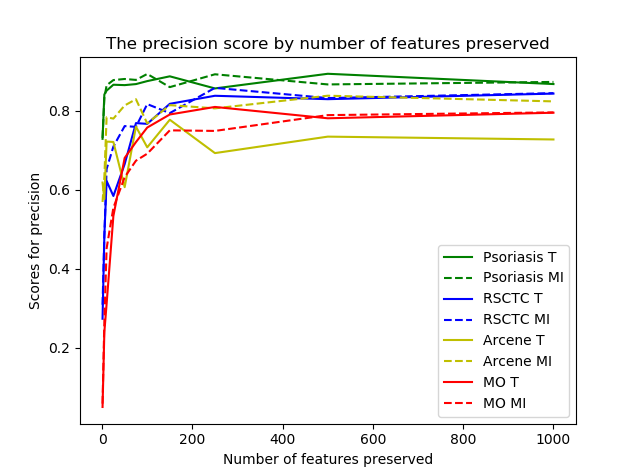
\includegraphics[width=0.7\textwidth]{Data_Rank_Prec_Scores.png}
		\caption{The average precision shown per dataset and rank.}
		\label{fig:DatasetRankPrecisionScores}
	\end{figure}

	% Insert figures
	\begin{figure}[H]
		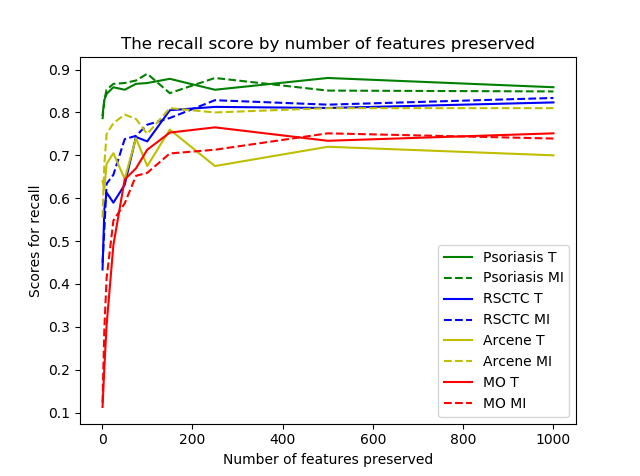
\includegraphics[width=0.7\textwidth]{Data_Rank_Rec_Scores.png}
		\caption{The average recall shown per dataset and rank.}
		\label{fig:DatasetRankRecallScores}
	\end{figure}